%% ----------------------------------------------------------------
%% InvestigationVision.tex
%% ---------------------------------------------------------------- 
\chapter{Vision Algorithms} \label{Chapter:InvestigationVision}

\section{Matching Algorithms}\label{Section:Comparison}
%\inote{find some references to back these claims up}
%\inote{Talk about how to compare images and TEST them all. Make a final comparison to decide on which will be used}
In computer vision, there are many different ways of comparing two similar images. These include the sum of absolute differences (S.A.D.) \citep{Hamzah:DistanceDetection}, the sum of squared differences (S.S.D.)\citep{Mrovlje:Distance_Stereoscopic} and  normalised cross correlation (N.C.C.)\citep{zhao2006image}. Each of these methods will be explained and tested to compare them. All testing will use images seen in figure \ref{fig:StereoTest}. Each test uses the same size template ($50\times50$) to compare the two images. 

\begin{figure}
\centering
\subfigure[Left Image]{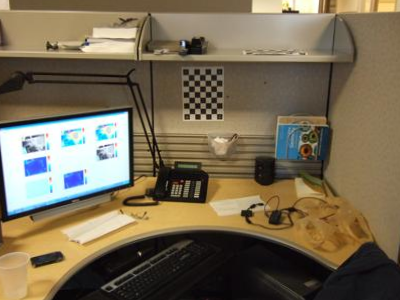
\includegraphics[scale=0.4]{./Figures/deskLeft.png} }
\subfigure[Right Image]{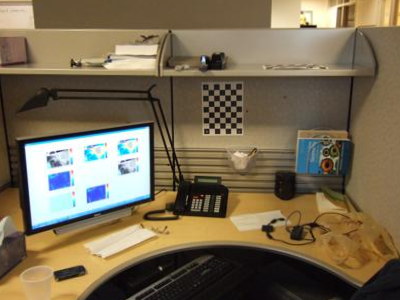
\includegraphics[scale=0.4]{./Figures/deskRight.png} }
\caption{Stereoscopic Test Images from MATLAB Examples}
\label{fig:StereoTest}
\end{figure}


%Explanation of how they work
%\inote{Maybe do a basic 5x5 example for each?}
\subsection{Sum of Absolute Differences}\label{Section:SAD}

Given two identically sized two dimensional matrices, $A, B$, of dimensions $I,J$, SAD is defined as
\begin{equation} \label{eq:SAD}
SAD = \sum\limits_{i=0}^{I-1} \sum\limits_{j=0}^{J-1} A[i,j] - B[i,j] 
\end{equation}

This method subtracts the observed template from the expected. All differences are then added together. This algorithm is simple and requires a small amount of computation. The algorithm returns values where a small result means the two images are well matched.

\subsection{Sum of Squared Differences}\label{Section:SSD}
\begin{equation}\label{eq:SSD}
SSD = \sum\limits_{i=0}^{I-1} \sum\limits_{j=0}^{J-1} (A[i,j] - B[i,j] )^2
\end{equation}

This is very similar to SAD but adds more complexity by squaring each difference. This removes the ability of equally different but opposite differences cancelling each other out (grey to white of one pixel will cancel out a white to grey difference in another with SAD). Again, a low result is a match in this case.

%\inote{sort chi out, if I want to do it...}
%\subsection{'Chi Squared'}
%$\chi ^{2}$ is ``Insert definition here". For use with images the equation can be adapted to \ref{eq:ChiSquare}. 
%
%\begin{equation} \label{eq:ChiSquare}
%\chi ^{2} = \sum\limits_{i=0}^{I-1} \sum\limits_{j=0}^{J-1}\frac{(A[i,j] - B[i,j])^2}{(A[i,j]+B[i,j])/2}
%\end{equation}


\subsection{Normalised Cross Correlation}\label{Section:NCC}
\begin{equation}\label{eq:NCC}
NCC =  \frac{1}{n}\sum\limits_{i,j} \frac{(A[i,j] - \bar{A}).(B[i,j] - \bar{B})}{\sigma _A . \sigma _B}
\end{equation}
\begin{center}
Where $n$ is the number of pixels in $A$ and $B$, \\$\sigma$ is the standard deviation of the image, and \\$\bar{A}$ is the a average pixel value. 
%\inote{Find a source for this equation}
\end{center}
%\inote{No date on Reference}
NCC is very similar to cross correlation, but normalised to reduce the error if one image is brighter than the other. This is common in computer vision \citep{Tsai:NCC} and cross correlation is a often used in digital signal processing, so fast algorithms have been made to calculate this. 

Unlike SSD and SAD, the normalised cross correlation gives a high value for a match. The downside to this algorithm comes with the complexity of the equation as it contains division and the calculation of the square root of a number in order to find the standard deviation. 
Floating point arithmetic is extensively used, which takes much more time to execute on a microcontroller than pure integer arithmetic.
%These operations are rarely implemented in hardware and are time consuming to carry out in software. They also require floating point registers and operates slowly on a microcontroller without any. 



%test and compare
\subsection{Comparison}

To compare these equations, a $50 \times 50$ template taken from the right picture was compared with the left image over the entire valid range. The coordinates on the graph give the centre pixel of the calculation. 

\begin{figure}
\centering
\subfigure[S.A.D Results. Blue shows areas of matching.\label{fg:Results:SAD}]{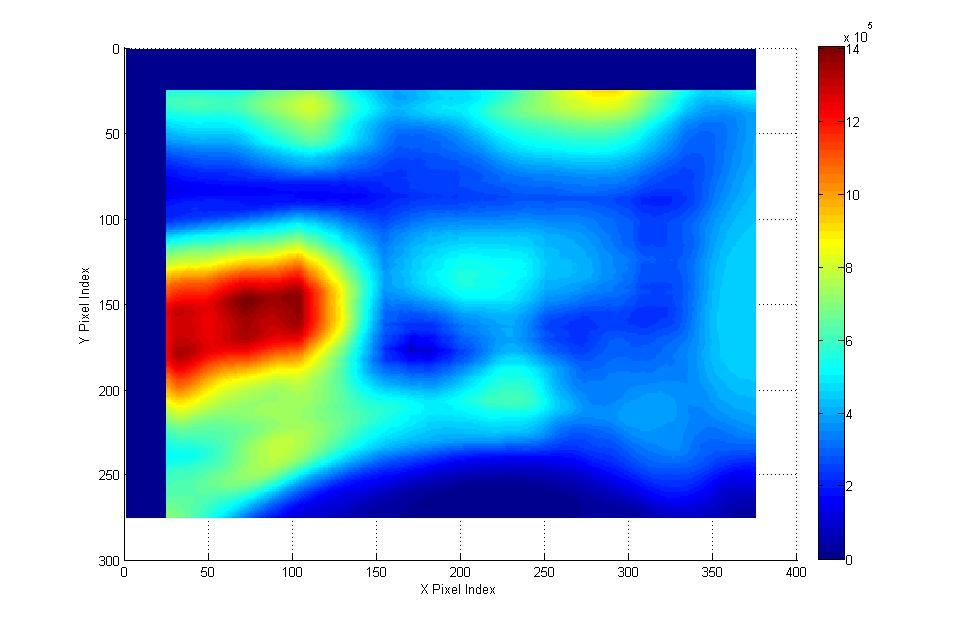
\includegraphics[width = 12cm, keepaspectratio]{./Figures/SADResults.eps} }
\subfigure[S.S.D. Results Blue shows areas of matching.\label{fg:Results:SSD}]{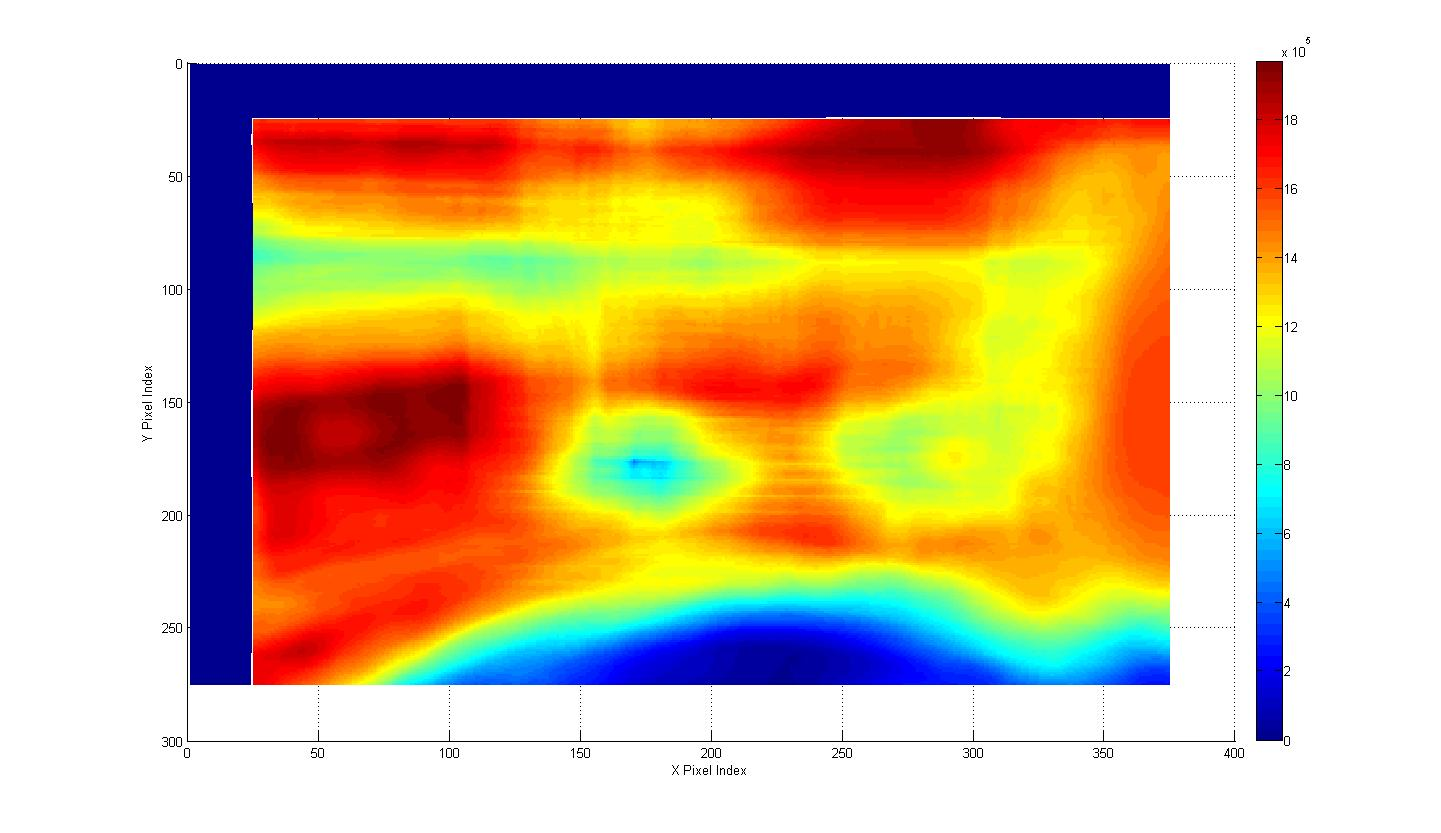
\includegraphics[width = 12cm, keepaspectratio]{./Figures/SSDResults.eps} }
\subfigure[N.C.C. Results Red shows areas of matching.\label{fg:Results:NCC}]{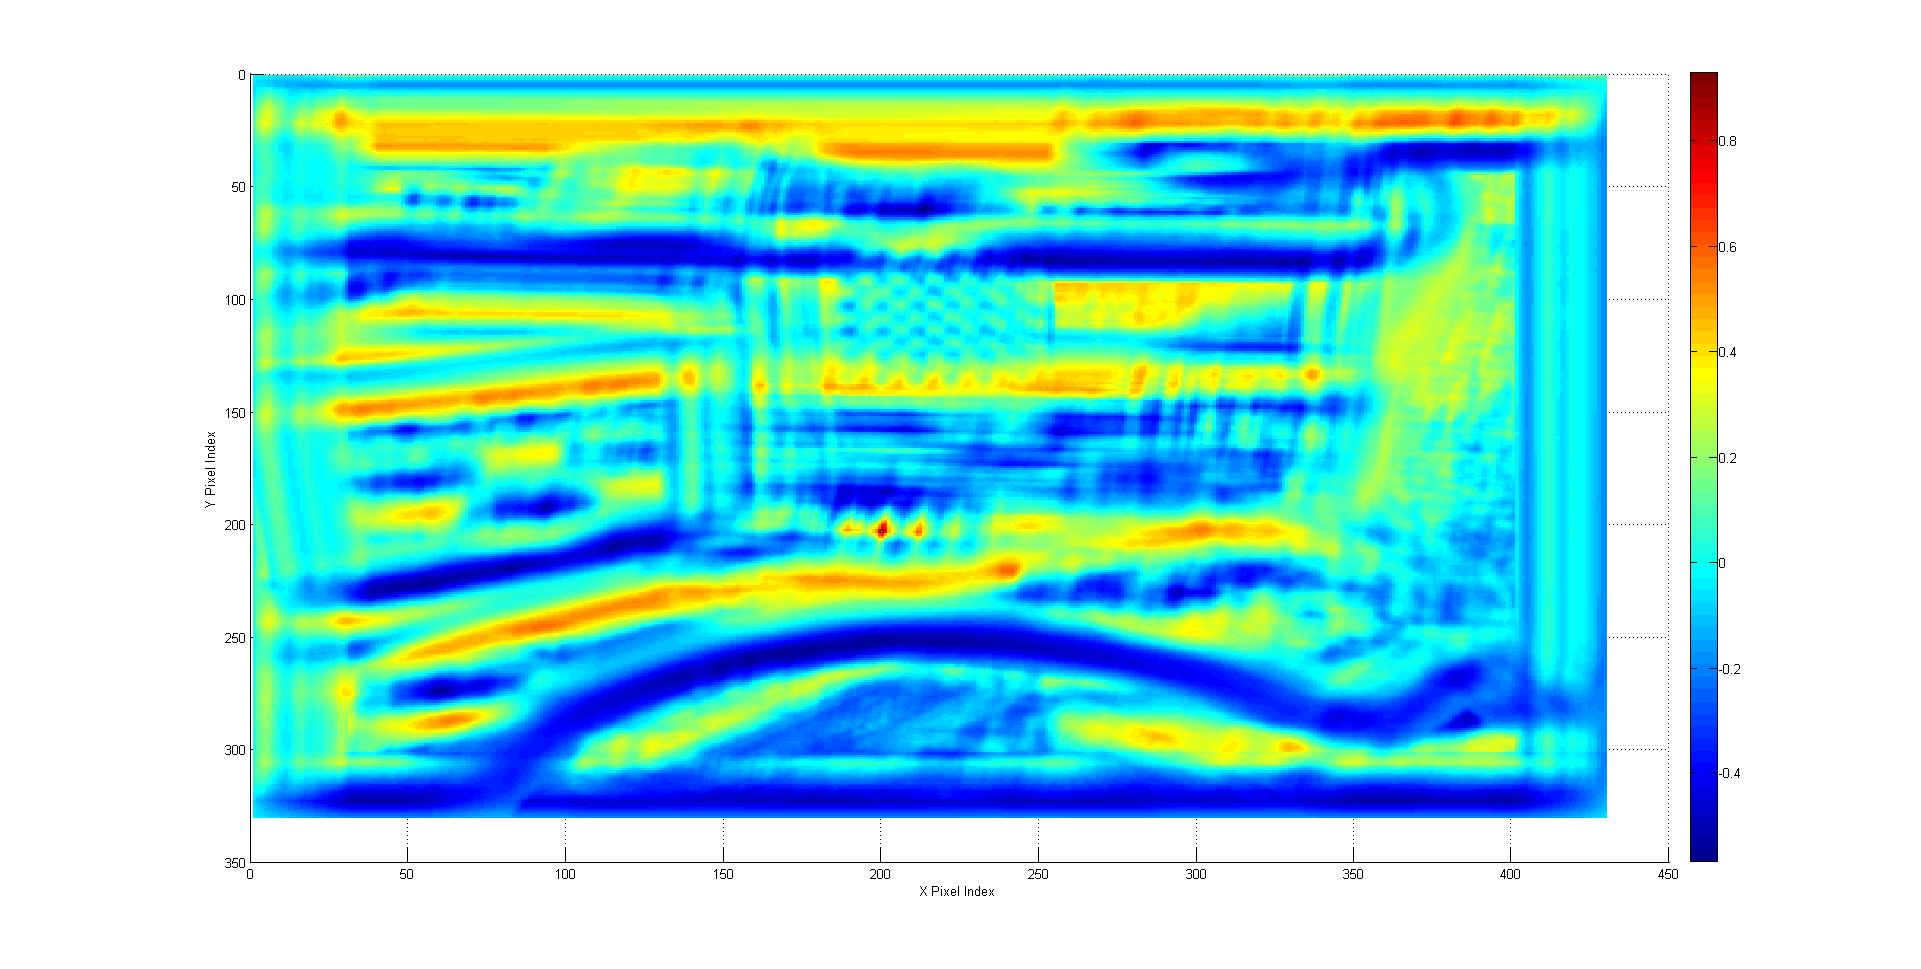
\includegraphics[width = 12cm, keepaspectratio]{./Figures/NCCResults.eps} }
\caption{Result Graphs of Comparison Algorithms}
\label{fg:CompResults}
\end{figure}

Each graph shows the correct area being identified as a match, but this also highlights the downfalls of the SAD and SSD. The graphs in figure \ref{fg:CompResults} are rotated to match the orientation of the images in figure \ref{fig:StereoTest}. Each of the images is tested by attempting to match the desk phone from the right image to the entirety of the left image. The actual match should be around $(170, 176)$. An exact result cannot be estimated as the images are not matched perfectly - there isn't an exact integer of pixel difference between the images. This is the sub pixel problem \citep{haller2012design}.

SAD results in figure \ref{fg:Results:SAD} show large areas of matching. A minimum occurs around the location expected($170,175$) of a value of $5.66\times 10^4$. 
However, the dark area beneath the desk causes a false detection. The SAD algorithm detects a greater comparison with a low value of $3370$ at $(227, 275)$ which causes a false match.
%However, along the bottom of the image, where a dark area occurs below the desk in the lower part of figures \ref{fig:StereoTest}, the SAD algorithm detects a greater comparison, with the lowest value in this area being $3370$ at $(227, 275)$. This creates a false detection here. 

SSD, figure \ref{fg:Results:SSD}, shows matches in the same two areas: where a match should occur and the dark area beneath the desk. The minimum value where the match should occur is $4.355 \times 10^5$ at location $(170,176)$. However, there is a large match correlation between the dark area under the desk where the actual lowest value of $2.768\times10^4$ occurs at $(225,274)$. This, again, is a false match and is a downfall of this algorithm.

The NCC results are visible in figure \ref{fg:Results:NCC}. A match can be seen at coordinate $(195,201)$ with a peak value of $0.9654$. The coordinate is different to the previous results because the cross correlation works over the boundary of the image creating more results. The dimensions of the image are $300 \times 400$, but the NCC returns an data set of dimensions $350 \times 450$ when using a template size of $50\times 50$. To get the actual match, half of the box size must be subtracted from the returned coordinate. This means the match occurs at $(170,176)$. With this algorithm, there is no area of the image which is close to a false detection. 

\subsection{Conclusion}
It can be seen that there is a direct correlation between the complexity of the matching algorithm to the reliability of the match returned. In brightly lit, colourful environments absent of dark colours, SAD and SSD should provide a reliable result, but this cannot be guaranteed to always be the case. Therefore further development of the matching algorithm will start with using the normalised cross correlation. A comprise between complexity and reliability needs to be reached, where reliability is the more desirable of the two. Cross correlation is also widely used in digital signal processing, so optimised algorithms suitable for microcontrollers do exist.

\section{Range Finding}
\subsection{Derivations}

By using two images separated by a horizontal distance, $B$, the range of an object can be found given some characteristics of the camera. Appendix \ref{Appendix:Range} contains the derivations for the follow scenarios:

\begin{enumerate}
\item Object is between the cameras (Figure \ref{problem_between})
\item Object is in left or right hand sides of both images (Figure \ref{problem_toleft})
\item Object is directly in front of a camera (Figure \ref{fig:problem_infront})
\end{enumerate}


\subsection{Summary}
There are three situations that can occur. These are listed below with their equations.

Object is between the two cameras:
\begin{equation} \label{eq:summary:1}
D = \frac{Bx_0}{2\tan(\frac{\varphi_0}{2})(x_1 - x_2)}
\end{equation}

Object is to the same side in both images:
\begin{equation} \label{eq:summary:2}
D = B.\frac{\cos(\varphi_2).\cos(\varphi_1)}{sin(\varphi_2 - \varphi_1)}
\end{equation}
Object is directly in front of a camera:
\begin{equation} \label{eq:summary:3}
D = B \tan\left(\frac{\pi}{2} - \varphi_{2}\right)
\end{equation}

Where $\varphi_1$ is defined in equation \eqref{eq:p2:phi1} and $\varphi_2$ is defined in equation \eqref{eq:p2:phi2}.
\begin{equation} \label{eq:p2:phi1}
\varphi_1 = \arctan\left(\frac{2x_1}{x_0}\tan\left(\frac{\varphi_0}{2}\right)\right)
\end{equation}
\begin{equation} \label{eq:p2:phi2}
\varphi_2 = \arctan\left(\frac{2x_2}{x_0}\tan\left(\frac{\varphi_0}{2}\right)\right)
\end{equation}
When the images have been matched, these equations can be used to calculate the range to an object.

\subsection{Field of View}
%The field of view is an important characteristic to calculate distances and must be measured for the camera. 
The field of view is an important cariable that must be measured for the camera. Field of view was measured by placing a ruler at a distance in front of the camera and measuring the total distance seen across the image. Equation \eqref{eq:FoV} was then used to calculate the field of view. This was done multiple times for accuracy. Results can be seen in table \ref{table:fieldofview}. The field of view used is the average of the data set and was found to be $\varphi_0 = 0.6249^c$. 
\inote{Figure to show this?}
\begin{equation}\label{eq:FoV}
\varphi_0 = 2\arctan\left(\frac{L}{2D}\right)
\end{equation}
\begin{table}
\caption{Table of results to calculate the field of view of the camera}
\label{table:fieldofview}
\centering
\begin{tabular}{|c|c|c|} \hline
L (mm) & D (mm) & $\varphi (^c)$ \\ \hline
70 & 104 & 0.6435\\
90 & 135 &0.6015\\
178 & 285 &0.6054\\
214 & 345 &0.6493 \\ \hline
\multicolumn{2}{|c|}{Average} & 0.6249 \\ \hline
\end{tabular}

\end{table}



\subsection{Testing}
MATLAB was used to test the range finding. It is unable to automatically detect an object so the user must select the template when prompted. 

A stereo pair of images of a rubber duck at different ranges were captured using the completed robot. To calculate the distance, a template from the right image of the ducks head was cross correlated with the left image. The maximum peak in the result was found and used as the match point. The distance was then calculated using equation \eqref{eq:summary:1}, with $B=42mm$, $\varphi_0=0.6249$ and $x_0=320$. Example images can be seen in figure \ref{fig:duck:stereo} and an example NCC result can be seen in figure \ref{fig:duck:ncc}. 

Table \ref{table:range} shows the distances tested with the distance calculated using the above method. The ranges calculated were inaccurate. This could be attributed to the resolution of the camera being low, so one pixel change can potentially be a large distance error. Matching can only be done to the accuracy of a few pixels without a more complex design and therefore can introduce a small error and cause a large distance error in the calculation. 

\begin{table}
\centering
\caption{Results of range finding test}
\label{table:range}
\begin{tabular}{|p{3cm}|p{3cm}|p{3cm}|p{3cm}|} \hline
Actual Distance (mm) & Pixel Difference in Images (pixel) & Calculated Distance (mm) & Error (\%) \\ \hline
100 & 290 & 72 & 28\\ 
200 & 152 & 137 & 32\\ 
300 & 109 & 191 & 36\\ 
400 & 88 & 236 & 41\\ 
500 & 75 & 277 & 45\\ 
600 & 67 & 310 & 48\\ 
700 & 61 & 341 & 51\\ 
800 & 57 & 365 & 54\\ 
900 & 53 & 393 & 56\\ 
1000 & 51 & 408 & 59\\ \hline
\end{tabular}
\end{table}
\begin{figure}
\centering
\subfigure[Left Image]{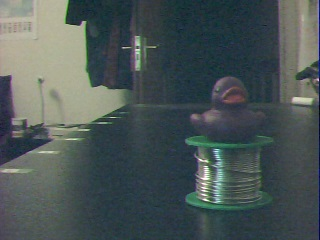
\includegraphics[scale=0.4]{./Figures/Duck_L.jpg} }
\subfigure[Right Image]{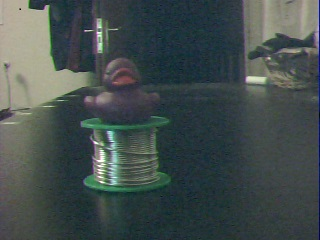
\includegraphics[scale=0.4]{./Figures/Duck_R.jpg} }
\caption{Stereo pair of images of a rubber duck on a reel of solder}
\label{fig:duck:stereo}
\end{figure}


\begin{figure}
\includegraphics[width=\textwidth]{Figures/NCC_Duck.eps}
\caption{NCC results from matching using the ducks head from the right image as the template to the left image}
\label{fig:duck:ncc}
\end{figure}

\subsection{Conclusion}

Extensive testing of the effect of separation of the cameras has been done before \citep{Mrovlje:Distance_Stereoscopic}. Figure \ref{fig:B:Plot} shows that by increasing $B$ will give you a larger range of detectable distances, but with a larger potential error with a low resolution camera. A separation of more than 100 pixels will result in around the same calculated distance due to the function being of the form $D =kx^{-1}$. This gives a range of distances that the can be detected. For $B=42mm$, it is around $200mm$ to $1m$. An external frame could be made to mount the cameras with a greater separation distance to alter this characteristic on the robot.

The robot was designed to be small, and the cameras were chosen as a cheap alternative to more expensive products on the market. The test results show that using the cameras with a small separation and low resolution, the system is unable to accurately measure distances to objects seen. The separation of objects in the images is a reciprocal function and the data gathered in the test matches this characteristic, see figure \ref{fig:Distance:DeltaX}. This means the system can perceive depth from the separation of the objects, but not accurately calculate the distance. 

\begin{figure}
\includegraphics[width=\textwidth]{Figures/BPlot.eps}
\caption{3D Surface plot graph showing range of distances that can be calculated over a range of camera separation, B, values.}
\label{fig:B:Plot}
\end{figure}
\begin{figure}
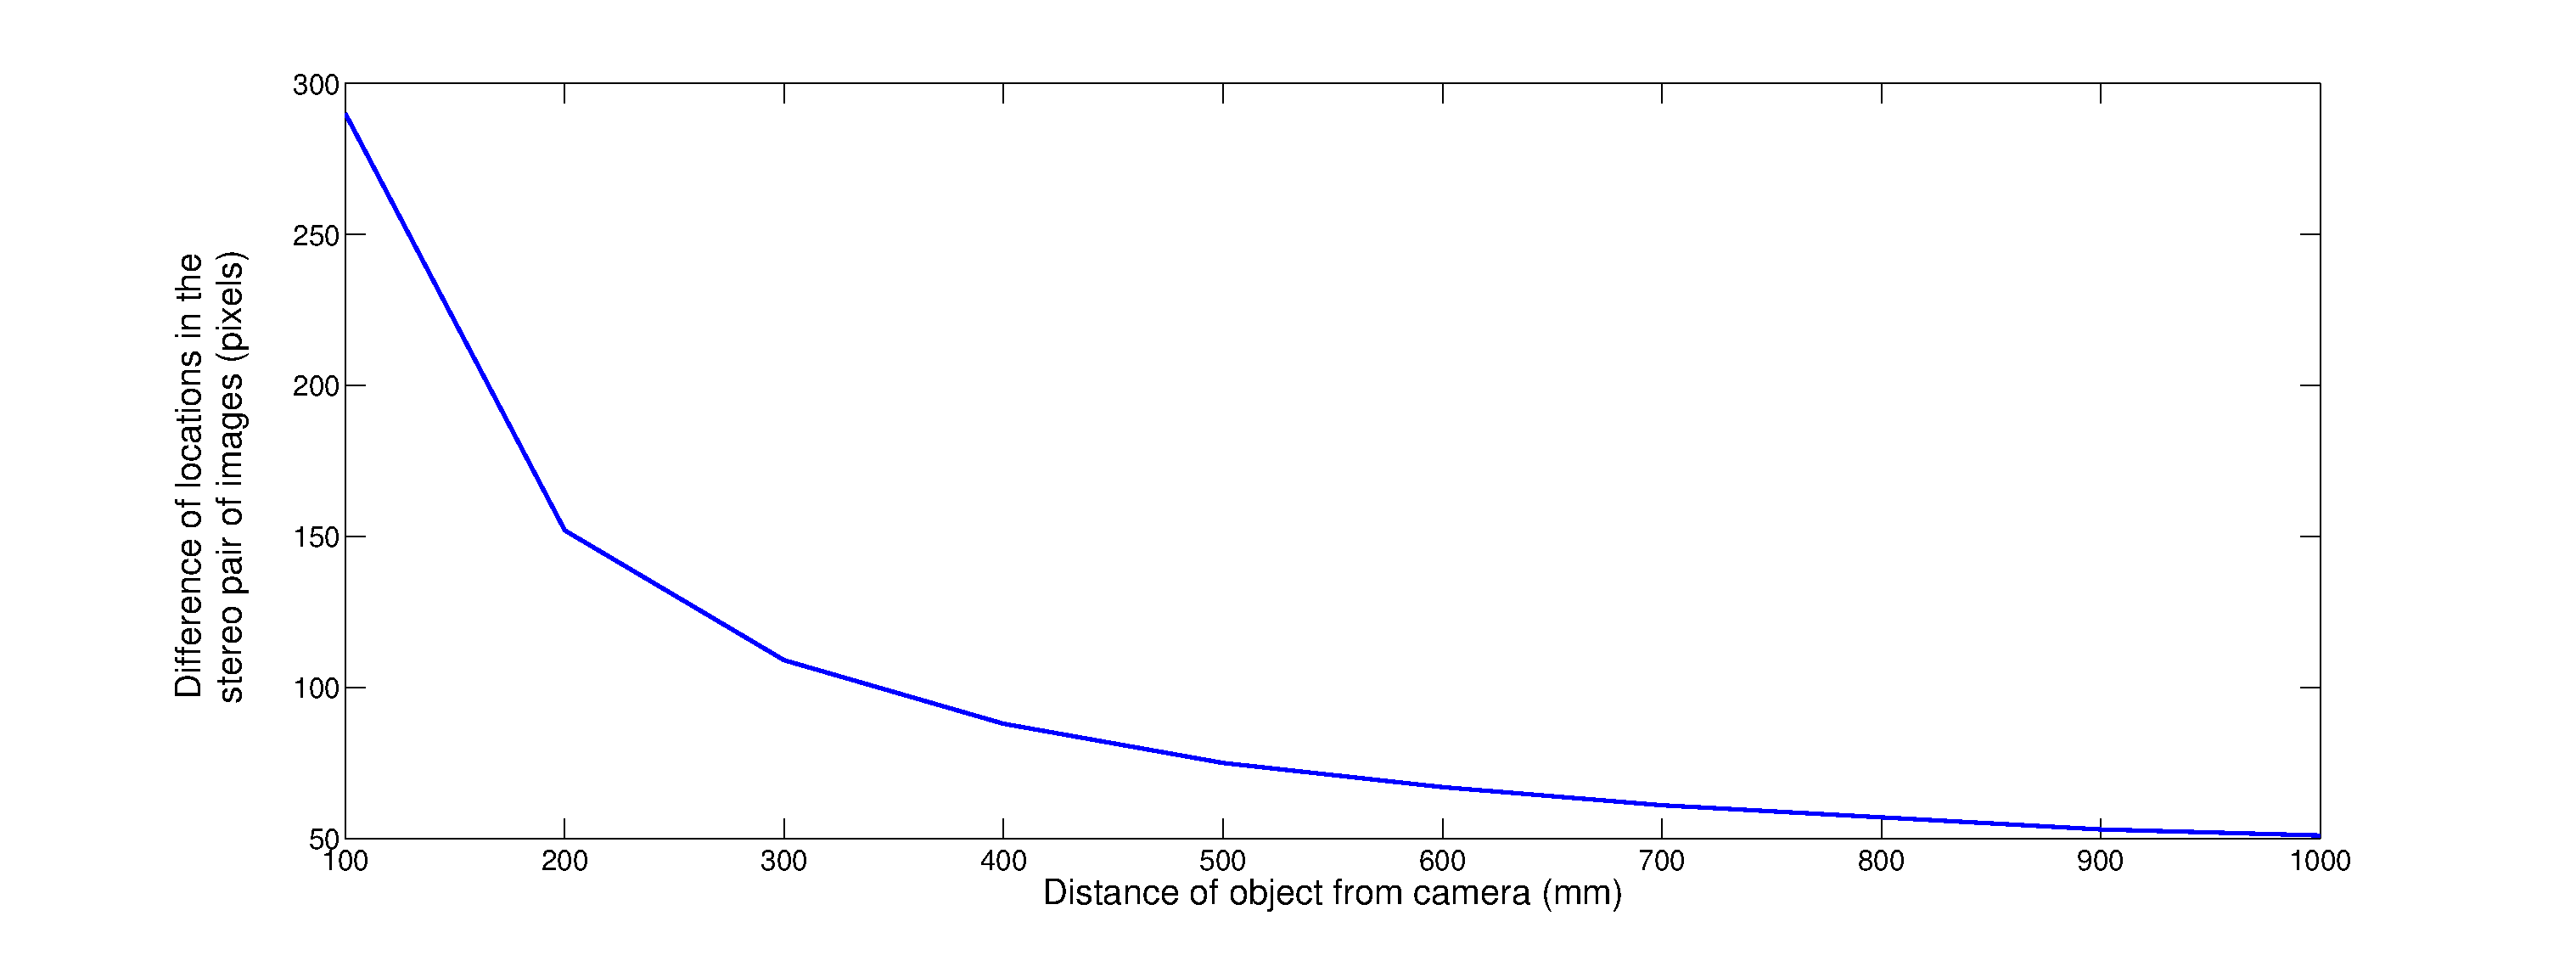
\includegraphics[width=\textwidth]{Figures/Distance_DeltaX.eps}
\caption{Graph showing Distance of the object against the difference in the match locations.}
\label{fig:Distance:DeltaX}
\end{figure}
\section{Fourier Transform}
\subsection{Background Research and the FFT}
The Fourier transform is a common tool in signal processing, used for filer design, system analysis and image processing as well as other applications. It transforms a time based signal to the frequency domain showing the frequency components contained in the signal as a complex number. This is often displayed as magnitude and phase. The Fourier transform is defined in equation \eqref{eq:fourier} and two examples of signals and their Fourier transforms are shown in figures \ref{fig:DiracFunctionFT} and \ref{fig:SquareWaveFT}. 
 
\begin{equation}\label{eq:fourier}
X(f) = \int\limits_{-\infty}^{\infty}x(t)e^{-\jmath 2 \pi ft}dt
\end{equation}

\begin{figure}
\centering
\subfigure[A graph showing a Dirac Function\label{fg:Dirac:Signal}]{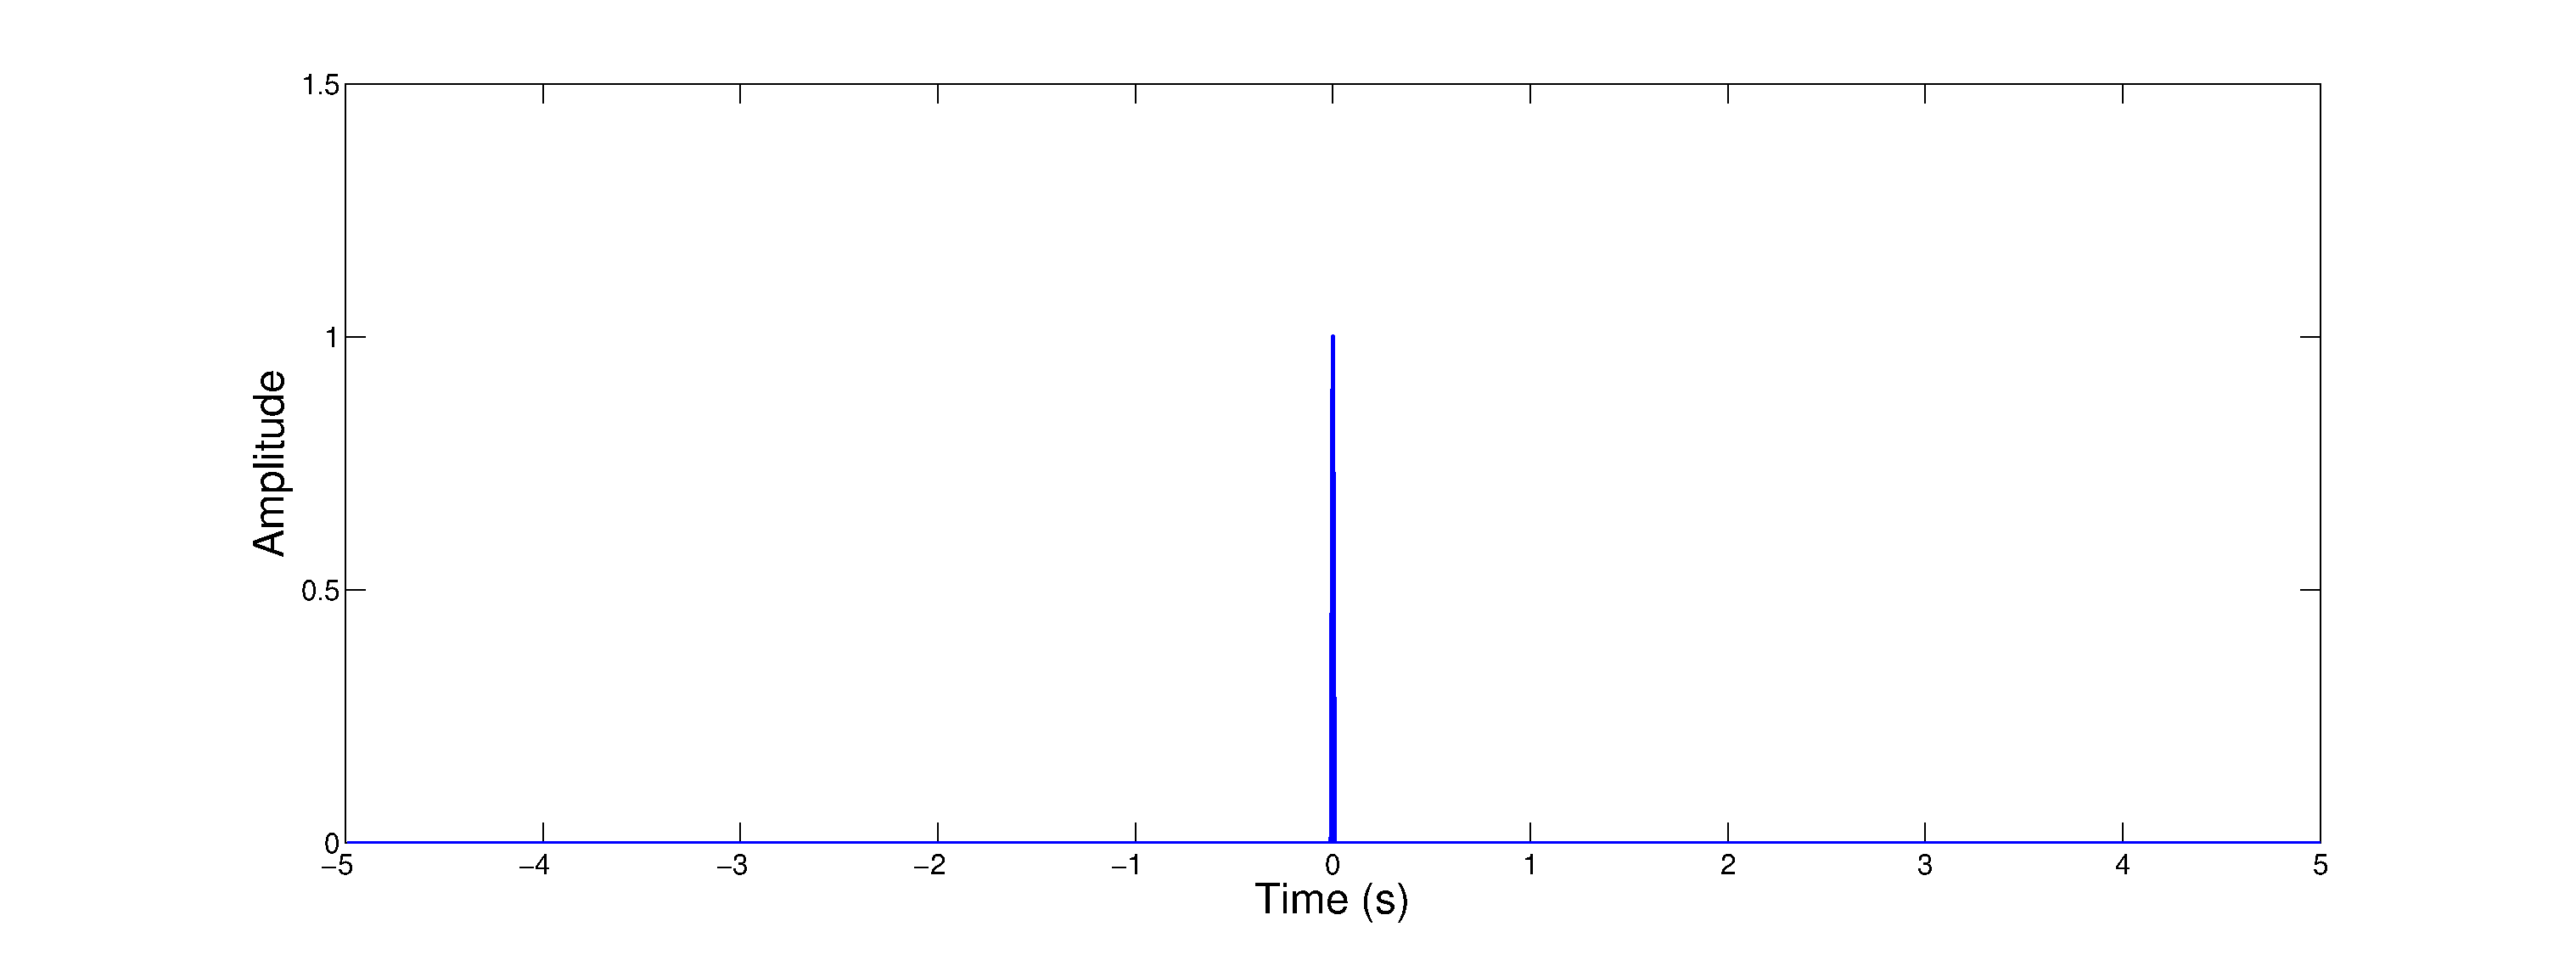
\includegraphics[width=\textwidth, keepaspectratio]{./Figures/Dirac_1D_Sig.eps} }
\subfigure[A graph showing the magnitude of the Fourier transform of the Dirac Function\label{fg:Dirac:Mag}]{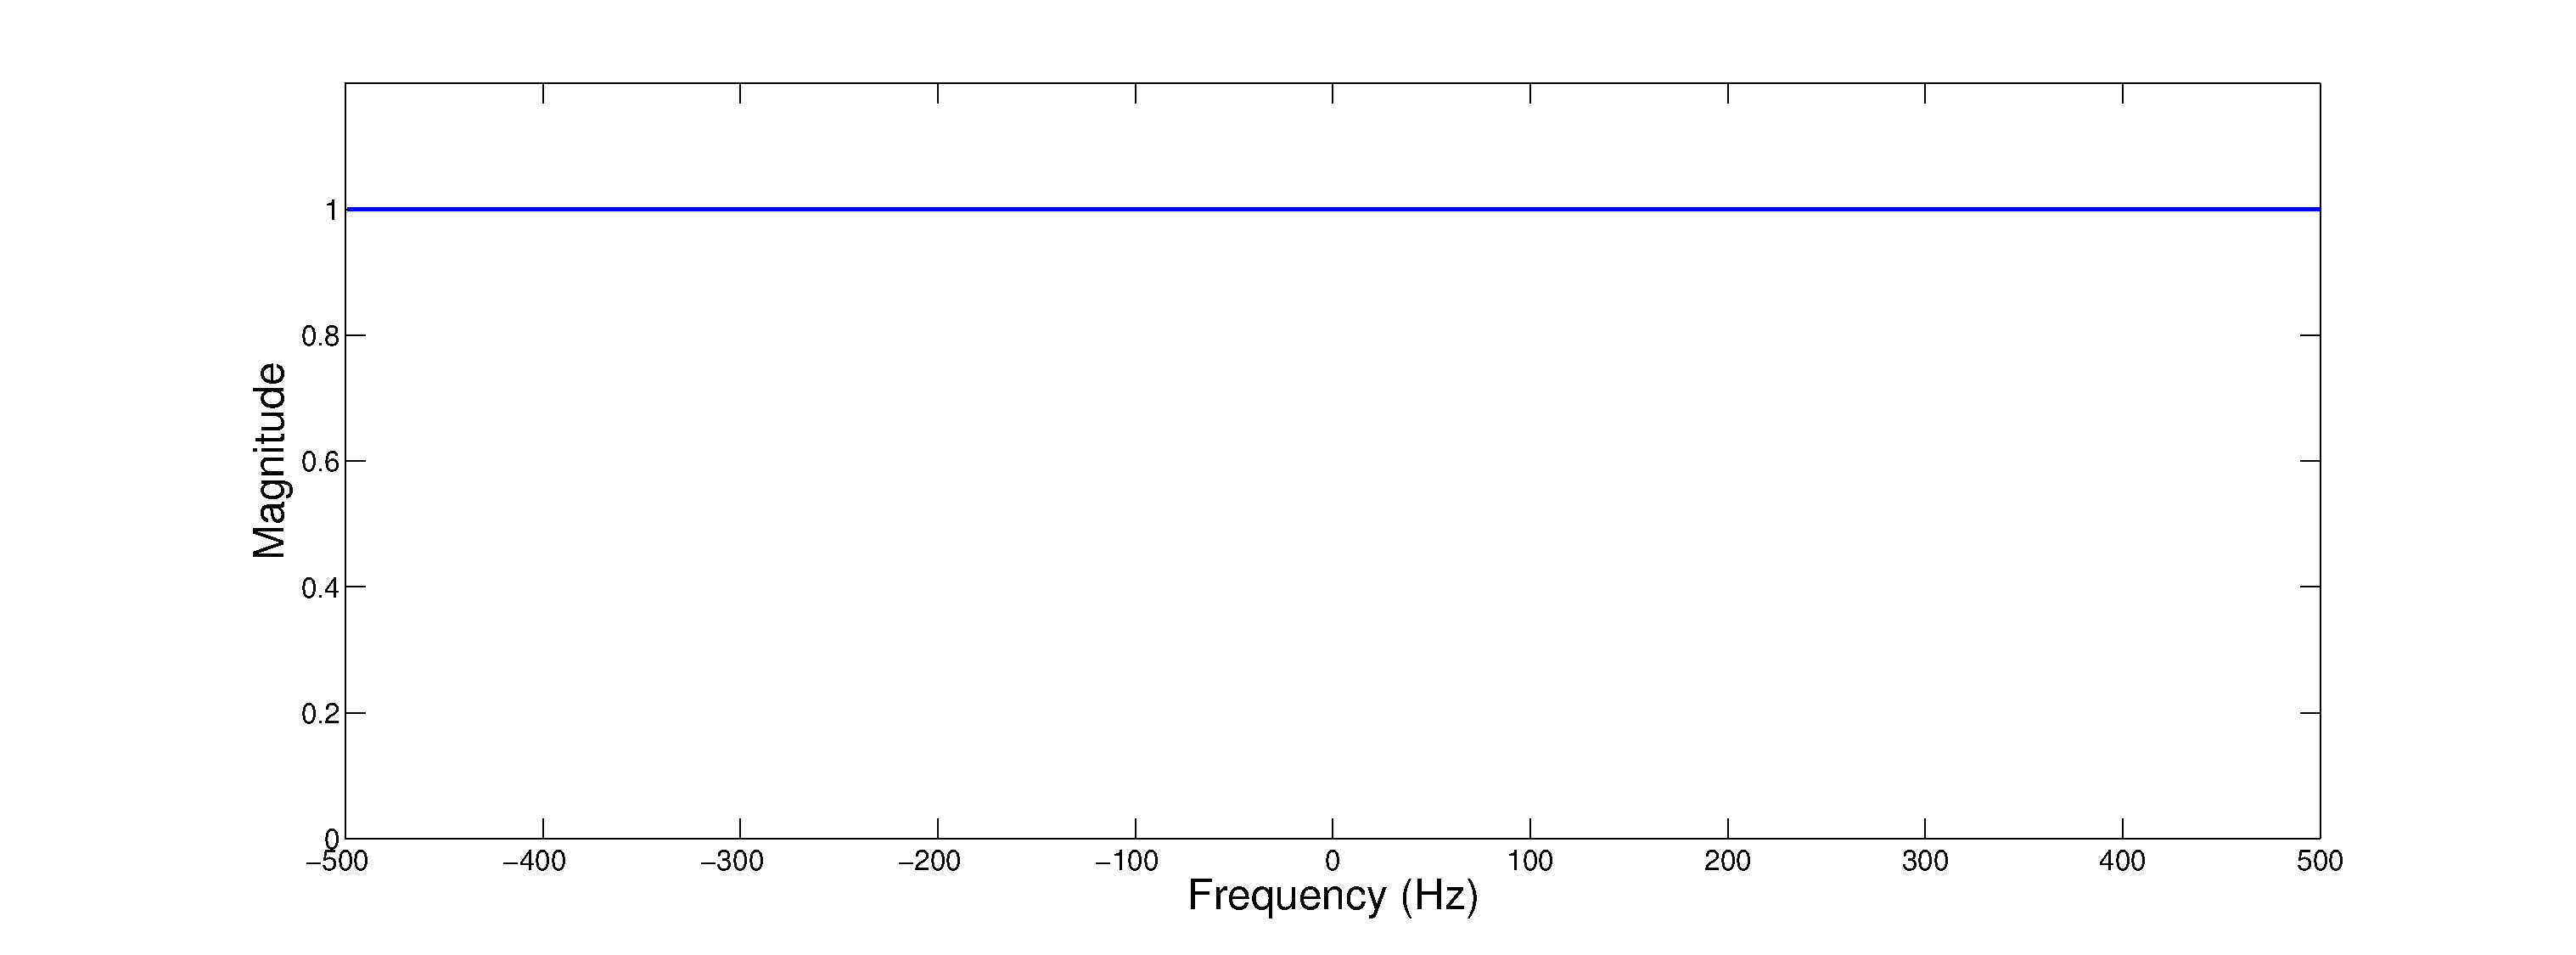
\includegraphics[width=\textwidth, keepaspectratio]{./Figures/Dirac_1D_Mag.eps} }
\subfigure[A graph showing the phase of the Fourier transform of the Dirac Function\label{fg:Dirac:Phase}]{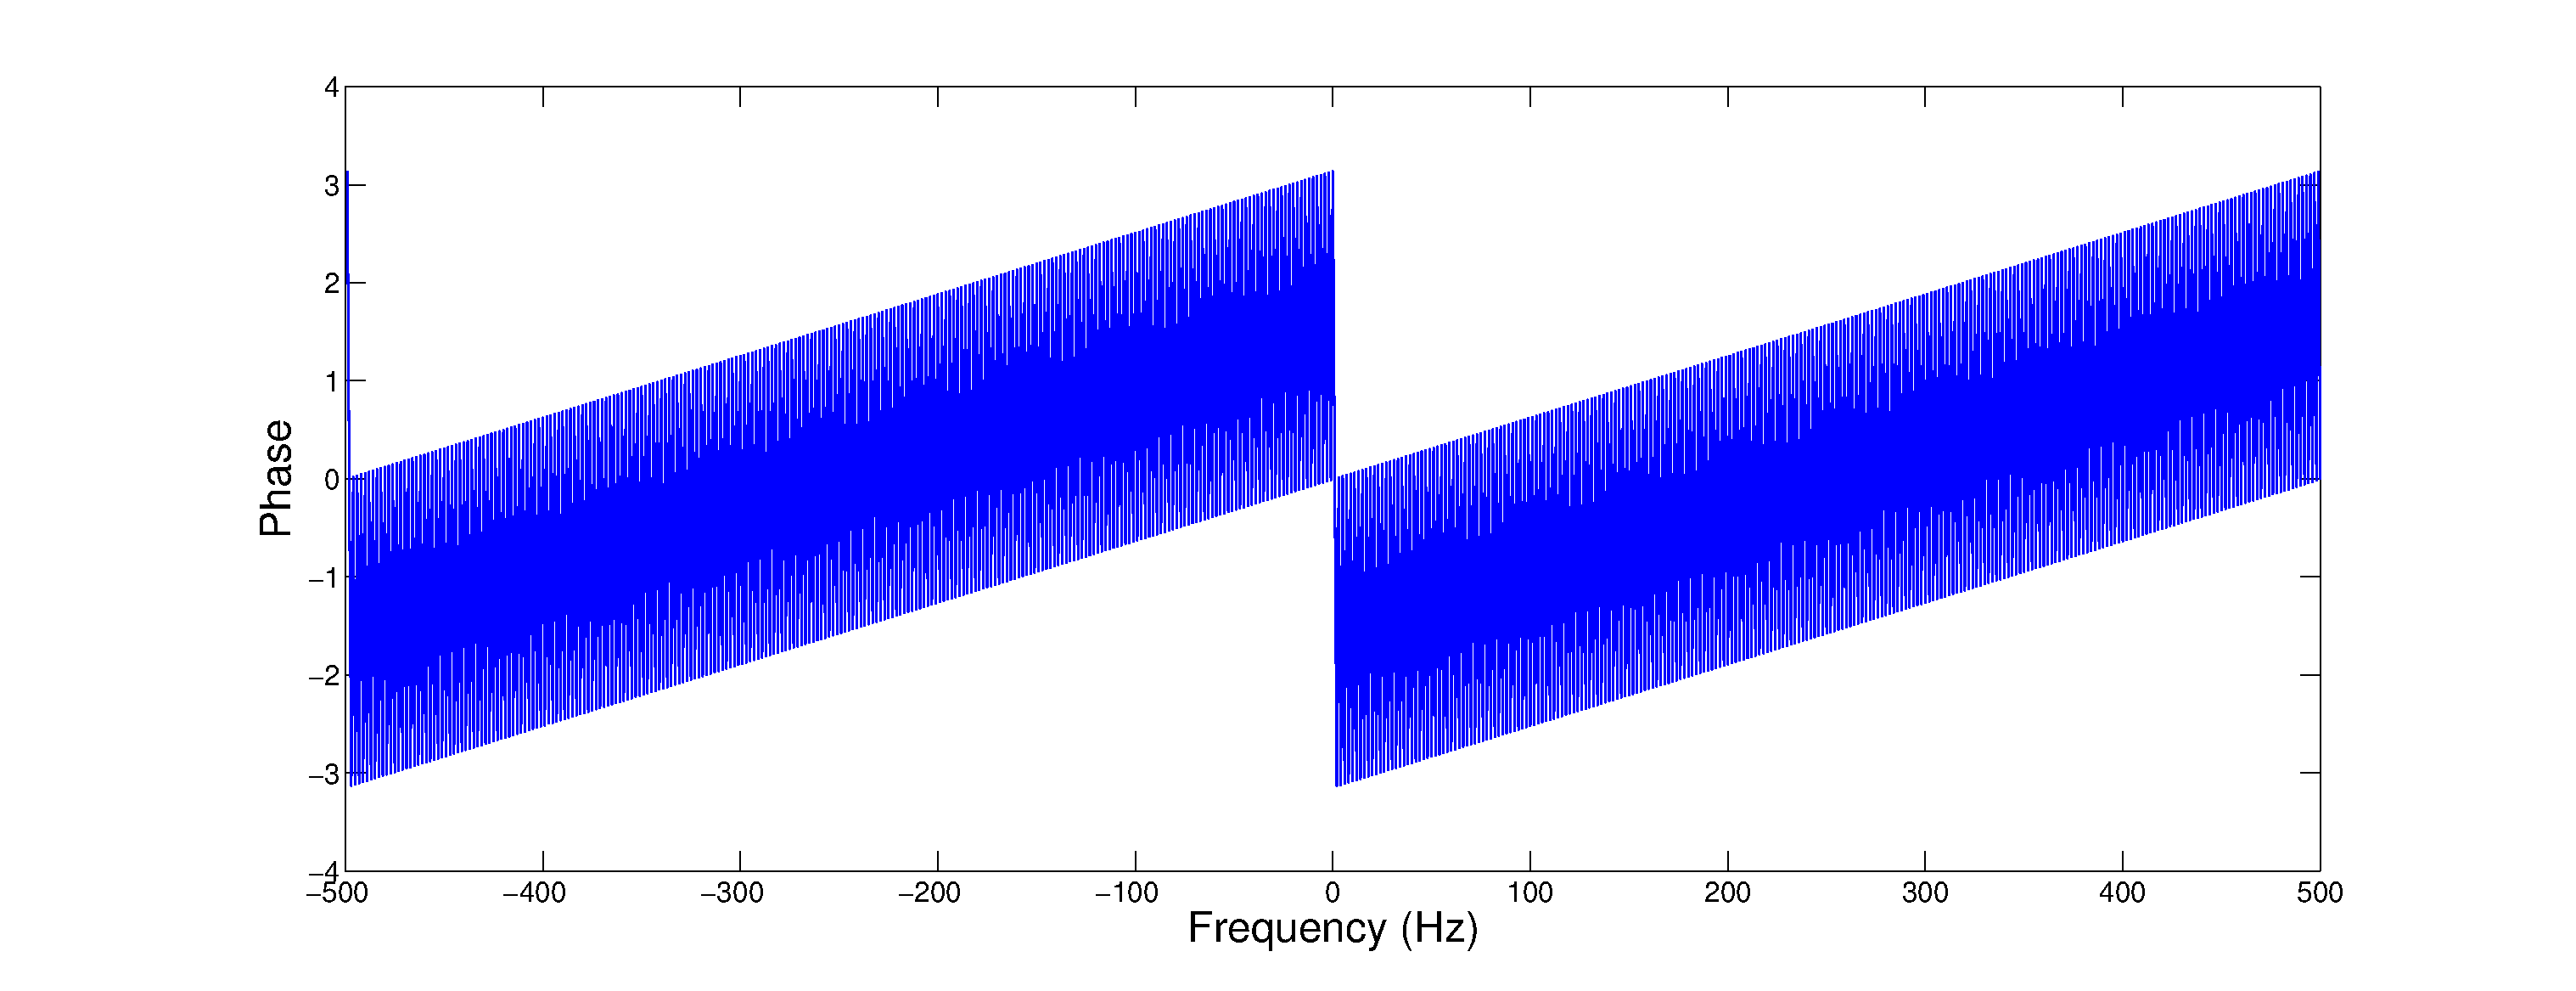
\includegraphics[width=\textwidth, keepaspectratio]{./Figures/Dirac_1D_Phase.eps} }
\caption{A Dirac signal and the phase and magnitude of its Fourier Transform}
\label{fig:DiracFunctionFT}
\end{figure}

\begin{figure}
\centering
\subfigure[A graph showing rectangular pulse\label{fg:Square:Signal}]{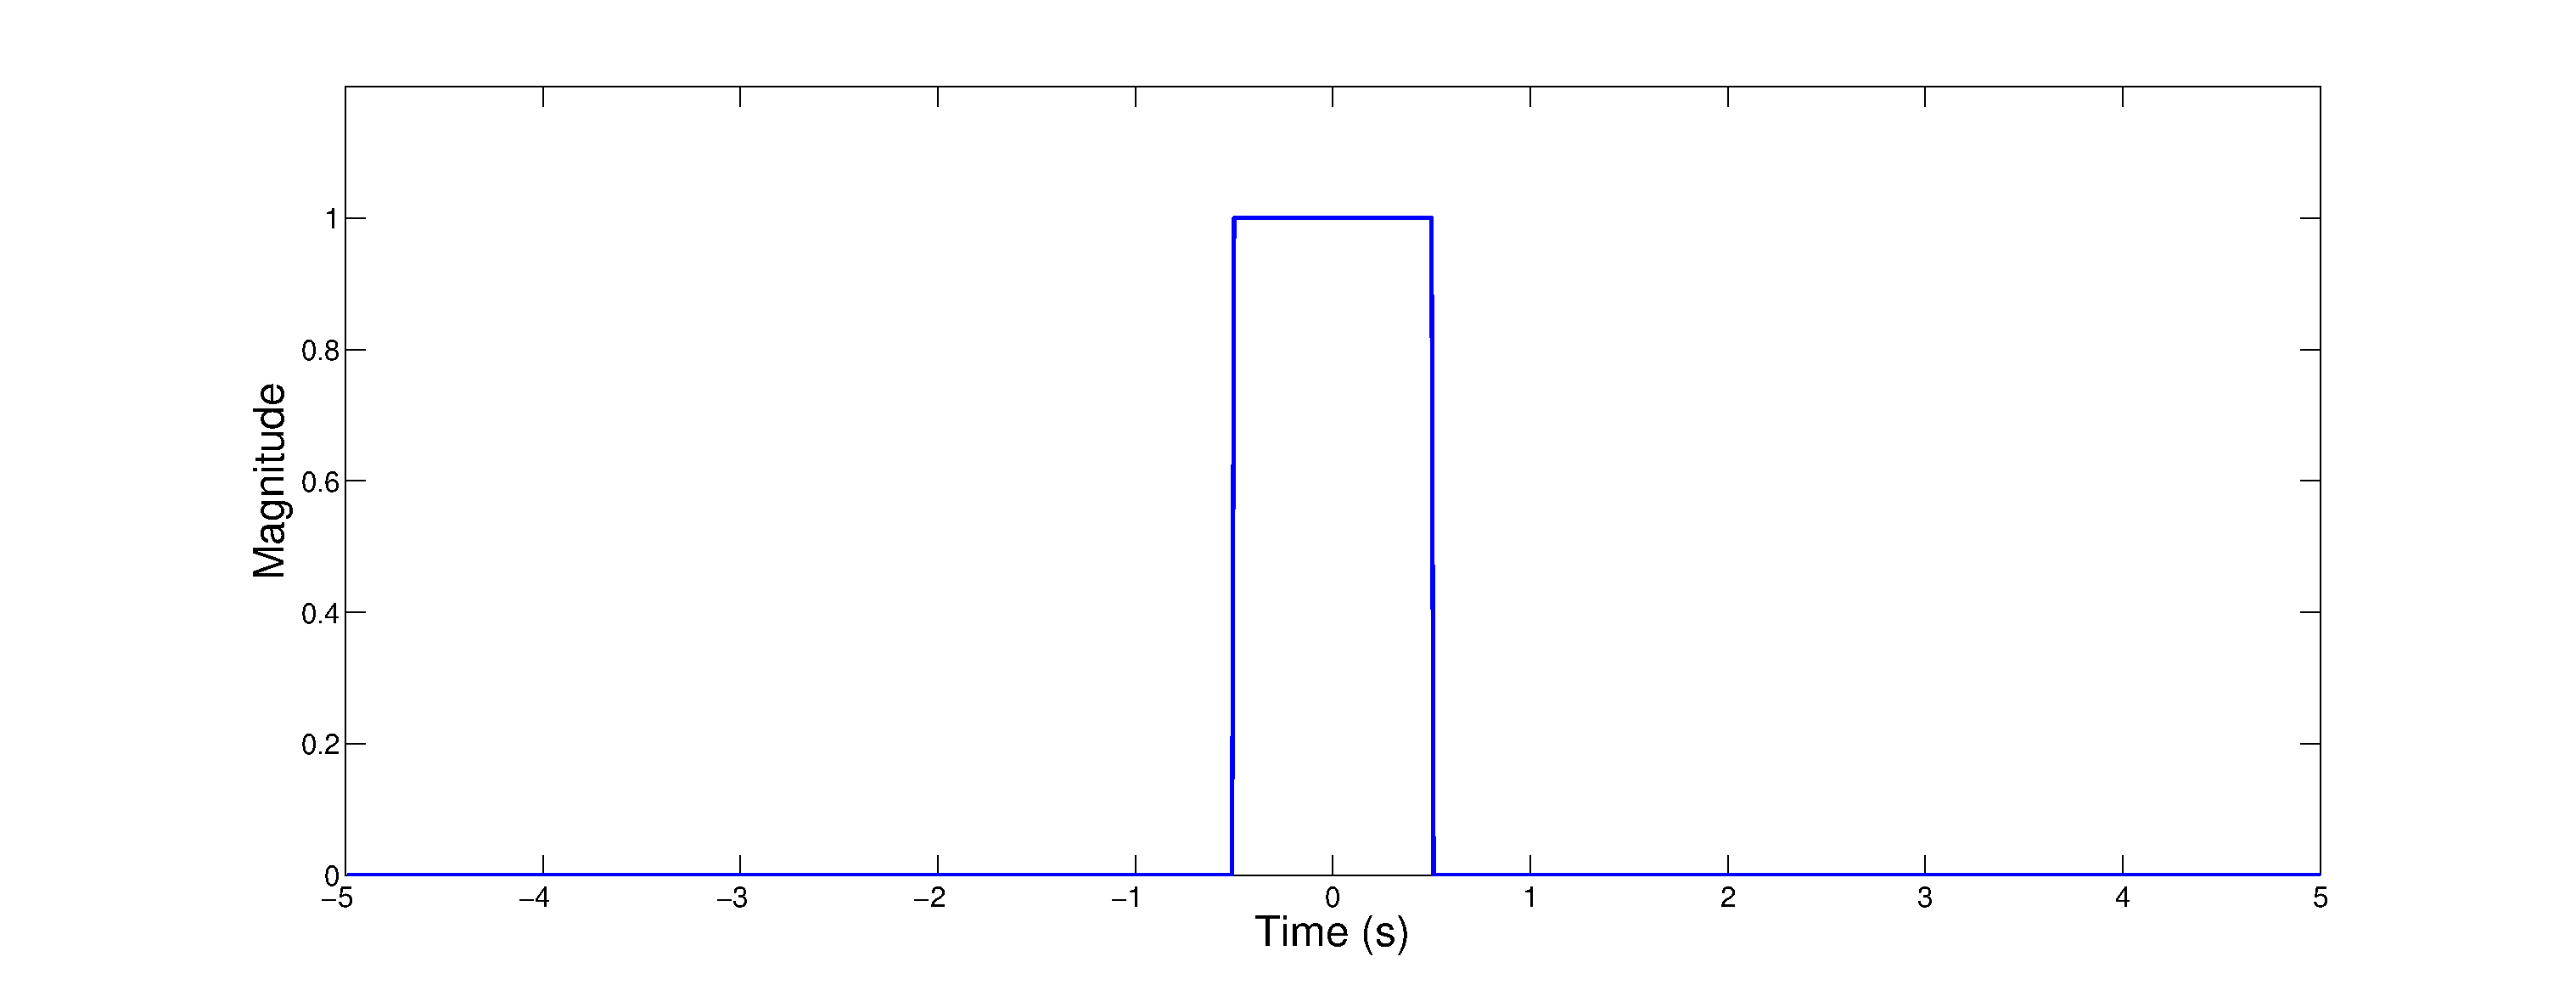
\includegraphics[width=\textwidth, keepaspectratio]{./Figures/Square_1D_Sig.eps} }
\subfigure[A graph showing the magnitude of the Fourier transform of the rectangular pulse\label{fg:Square:Mag}]{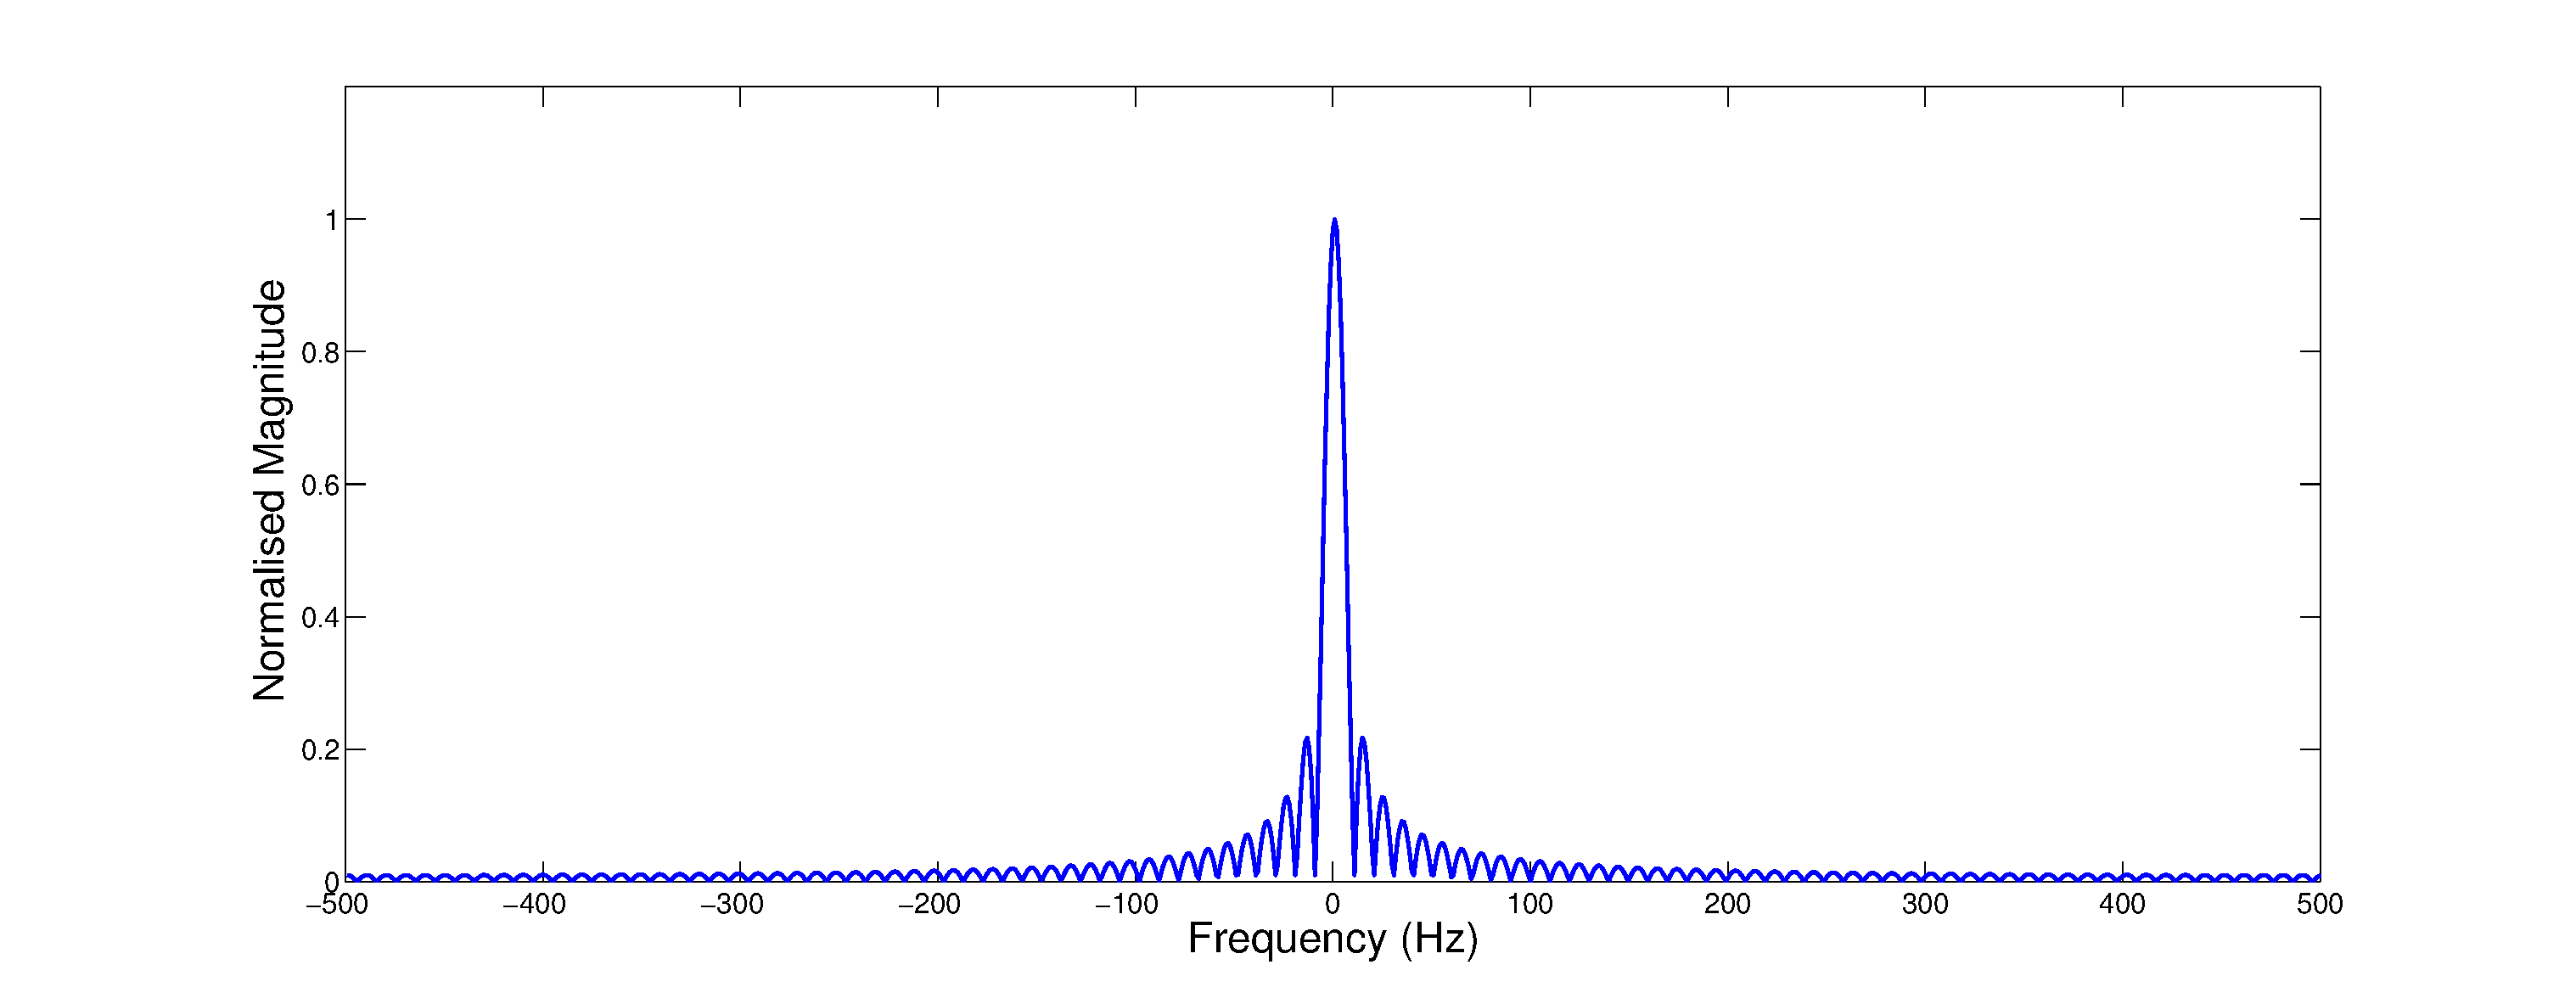
\includegraphics[width=\textwidth, keepaspectratio]{./Figures/Square_1D_Mag.eps} }
\subfigure[A graph showing the phase of the Fourier transform of the rectangular pulse\label{fg:Square:Phase}]{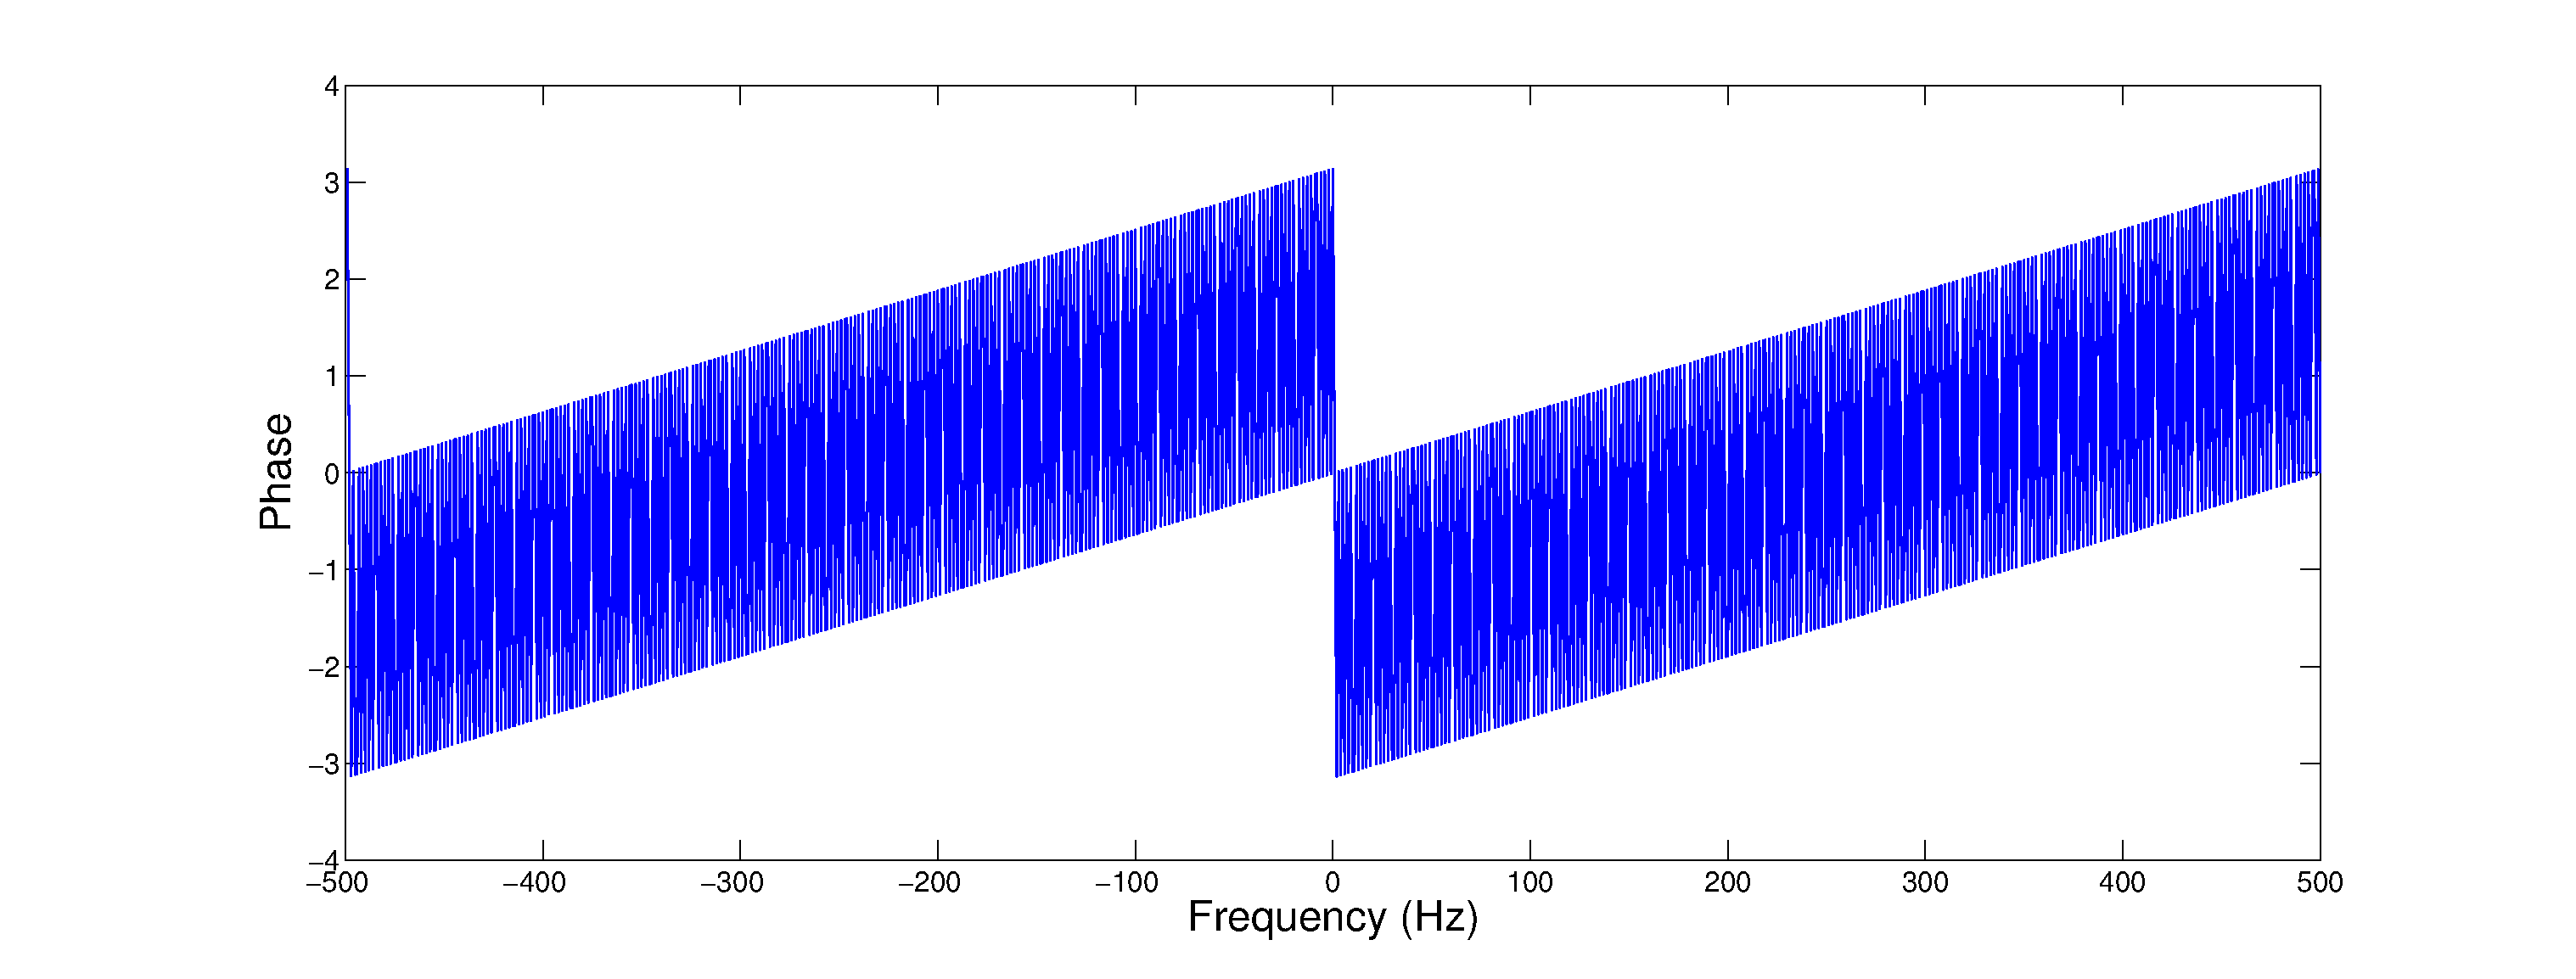
\includegraphics[width=\textwidth, keepaspectratio]{./Figures/Square_1D_Phase.eps} }
\caption{A 2D Rectangular pulse and the phase and magnitude of its Fourier Transform}
\label{fig:SquareWaveFT}
\end{figure}

The equation for the Fourier transform in equation \eqref{eq:fourier} is for continuous time. A discrete Fourier transform (DFT) exists for finite, equally spaced samples. This is commonly used in digital systems and is defined in equation \eqref{eq:DFT}. There exists a Fast Fourier transform (FFT) which gives exactly the same results as the DFT, but is optimised in terms of number of multiplications done. The FFT is most suitable for use on microcontrollers due to the speed of calculation and the availability of code extracts. %The FFT will be used in implementation due to availability of code and speed of use. 

\begin{equation}\label{eq:DFT}
X[k] = \sum\limits_{0}^{N-1}x[n]e^{-\jmath \Omega_0 kn}
\end{equation}
\begin{center}
Where $\Omega_0$ is the sample frequency
\end{center}

A property of the Fourier transform of interest is the convolution theorem which states that convolution in time is multiplication in frequency and is defined mathematically in equation \eqref{eq:ConvolutionMultiplication}. Cross correlation is defined in equation \eqref{eq:CrossCorrelation} and related to convolution by equation \eqref{eq:CrossCorrelation}. With images, $f(t)$ is a real signal, its conjugate is exactly the same, $f(t) \equiv f^*(t) \text{ given that} f(t) \in \Re$. Fourier transforms can be used to calculate cross correlation more efficiently, by multiplying the Fourier transform of an image by the reversed template.% This means that to compute a cross correlation, the Fourier transform of the image and the reversed template can be used and multiplied together. 


\begin{equation}\label{eq:ConvolutionMultiplication}
\int\limits_{-\infty}^{\infty}f(\tau)g(t-\tau)d\tau = f(t) \ast g(t) = X(f)\cdot Y(f)
\end{equation}
\begin{equation}\label{eq:CrossCorrelation}
\int\limits_{-\infty}^{\infty}f^*(\tau)g(t+\tau)d\tau = f(t) \star g(t) = f'(-t) \ast g(t) = X(-f)\cdot Y(f)
\end{equation}

%\begin{equation}\label{eq:CCtoConv}
%f(t) \star g(t) = f(t) \ast g(-t) = F(f) \cdot G(-f)
%\end{equation}

%\inote{example of convolution used as correlation. Include some pretty graphs}
\subsection{Two Dimensional Fast Fourier Transform}
A two dimensional (2D) Fourier transform exists for analysing 2D signals, such as an image. The Fourier Transform is shown in equation \eqref{eq:2dFT} and the discrete version is shown in \eqref{eq:2dDFT}

\begin{equation}\label{eq:2dFT}
F(u,v) = \frac{1}{2\pi}\int\limits_{-\infty}^{\infty}\int\limits_{-\infty}^{\infty}f(x,y)e^{-2\pi\jmath (xu+yv)}dxdy
\end{equation}
\begin{equation}\label{eq:2dDFT}
F(u,v) = \frac{1}{N} \sum\limits_{x=0}^{N-1}\sum\limits_{y=0}^{N-1}f(x,y)e^{-\frac{2\pi\jmath (xu+yv)}{N}} \; \; \; \; \; x,y,u,v \in \left\lbrace 0\dots N-1\right\rbrace
\end{equation}

Figures \ref{fig:2DDiracFunctionFT} and \ref{fig:2DSquareWaveFT} show the 2D equivalent test signals of figures \ref{fg:Dirac:Signal} and \ref{fg:Square:Signal} and the phase and magnitudes of their Fourier Transforms. There is a direct similarity between the 1D and 2D spectra; the magnitudes of the Dirac (figures \ref{fg:Dirac:Mag} and \ref{fg:Dirac2D:Mag}) are both constant values and the rectangular pulses both have a modulus sinc function magnitude (figures \ref{fg:Square:Signal} and \ref{fg:Square2D:Signal}). 

\begin{figure}
\centering
\subfigure[An image of a 2D Dirac Function\label{fg:Dirac2D:Signal}]{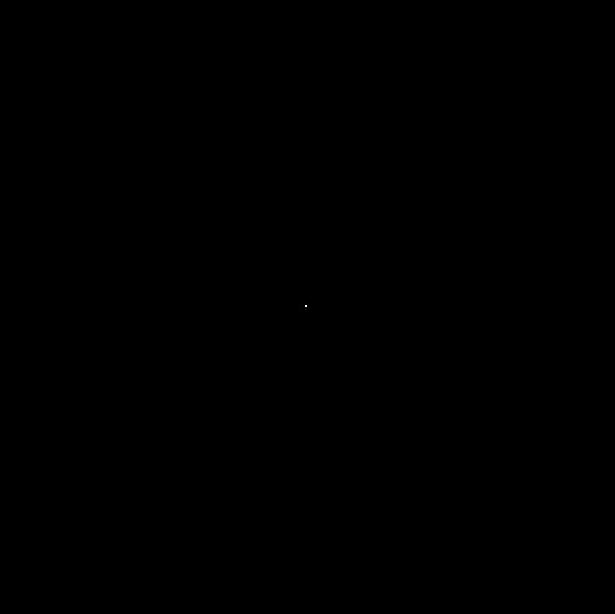
\includegraphics[width=10cm, keepaspectratio]{./Figures/Dirac_2D_Sig.jpg} }
\subfigure[An image of the magnitude of the Fourier transform of the 2D Dirac Function\label{fg:Dirac2D:Mag}]{\fbox{
\includegraphics[width=(\textwidth / 2)-1cm, keepaspectratio]{./Figures/Dirac_2D_Mag.jpg} }}
\subfigure[An image of the phase of the Fourier transform of the 2D Dirac Function\label{fg:Dirac2D:Phase}]{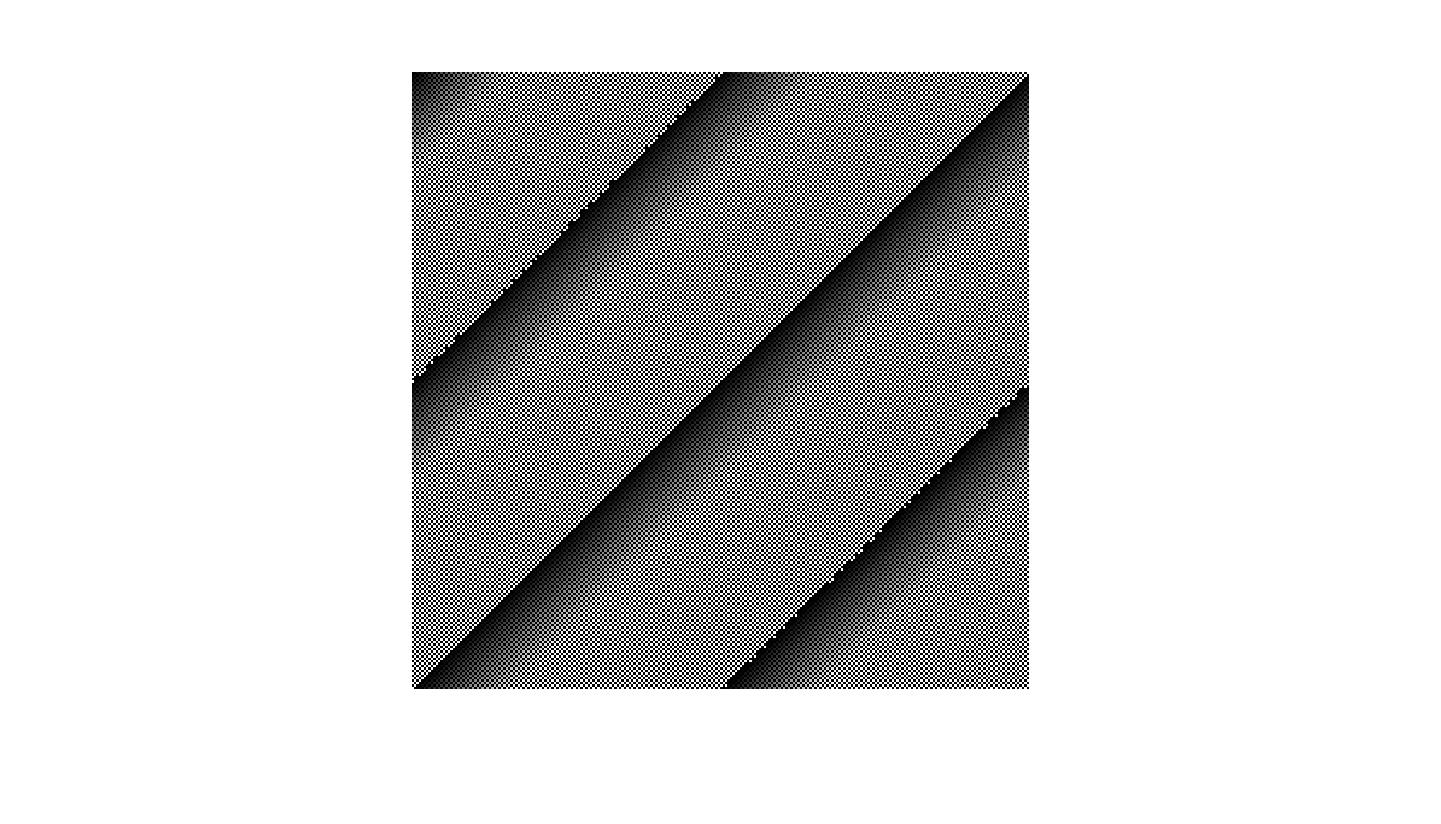
\includegraphics[width =(\textwidth / 2)-1cm, keepaspectratio]{./Figures/Dirac_2D_Phase.jpg} }
\caption{A 2D Dirac signal and the phase and magnitude of its Fourier Transform}
\label{fig:2DDiracFunctionFT}
\end{figure}

\begin{figure}
\centering
\subfigure[An image of the 2D rectangular pulse\label{fg:Square2D:Signal}]{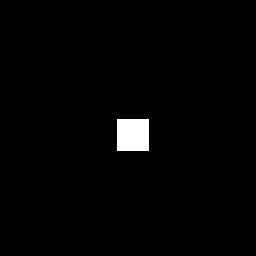
\includegraphics[width =10cm, keepaspectratio]{./Figures/Square_2D_Sig.jpg} }
\subfigure[An image of the magnitude of the Fourier transform of the 2D rectangular pulse\label{fg:Square2D:Mag}]{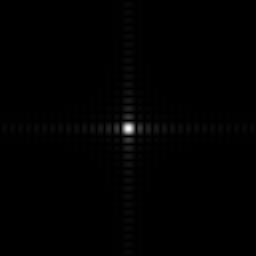
\includegraphics[width =(\textwidth / 2)-1cm, keepaspectratio]{./Figures/Square_2D_Abs.jpg} }
\subfigure[An image of the phase of the Fourier transform of the 2D rectangular pulse\label{fg:Square2D:Phase}]{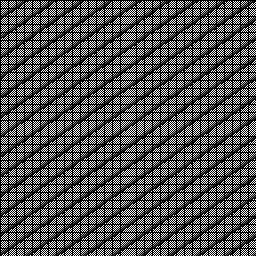
\includegraphics[width =(\textwidth / 2)-1cm, keepaspectratio]{./Figures/Square_2D_Phase.jpg} }
\caption{A 2D Rectangular Pulse signal and the phase and magnitude of its Fourier transform}
\label{fig:2DSquareWaveFT}
\end{figure}

The 2D Fourier transform can also be optimised to a FFT algorithm in a similar way as the 1D case. The algorithm, sometimes referred to as the Butterfly transform, is briefly discussed in \cite{nixon2012feature} where it is explained that the algorithm can be easily applied to images with equal dimensions that are a power of 2. The algorithm utilises the separability property of the Fourier transform. 

The 2D FFT can be implemented using a 1D FFT as follows:
\begin{enumerate}
\item Calculate the 1D FFT of each of the rows of the 2D data. (An FFT of data of length $n$ returns an array, also of length $n$)
\item Calculate the 1D FFT of each of the columns of the 2D data returned from the previous step.
\end{enumerate}
Total number of FFTs done is $2n$ where $n$ is the height/width of the image. 
\inote{Maybe make a figure to help explain?}
\subsection{Implementing the FFT}
%\inote{Include and explain code}
The Atmel Software Framework \citep{Atmel:ASF} included a digital signal processing library. This contained functions to compute the FFT of a real or complex array, the inverse FFT and the magnitude of complex data. Further restrictions are imposed by the DSP library used as the data must be an even power of 2, and that the data is in fixed point notation. This gives a usable dimension of $256 \times 256$ for processing images on the AVR. Though the height of an image from the OV7670 camera is $240$ pixels, the image can be transformed so that it repeats for 16 rows at the bottom as the Fourier transform works on an assumption of the data being periodic.

A function was made, called \textit{FFT2DCOMPLEX}, to realise the 2D FFT on the microcontroller. The FFT function requires the data to be 4 byte aligned (A\_ALIGNED) and of type \textit{dsp16\_complex\_t}. The data must be given in fixed point notation and it is returned in fixed point notation. A 16 bit representation was chosen over 32 bit due to being more functions for 16 bit data available. 


\subsection{Testing of the FFT on AVR}
\subsubsection{1D FFT Test}
A Dirac function and a rectangular pulse were used as test signals. 

Figure \ref{fig:AVR:FFT:Dirac:Input} shows the input signal given to the AVR. It is a 256 long array of a Dirac function. This was then converted to the internally defined fixed point notation and passed through the Fourier transform method. The resulting complex array was then saved to a Comma Separated Value file and read into MATLAB. Figure \ref{fig:AVR:FFT:Dirac:Output} shows the calculated phase and magnitude plots of the output complex array. The magnitude is relatively flat and around the value of 1. In comparison with figure \ref{fg:Dirac:Mag}, they are relatively similar. The phase, however, seems to be very different. Figure \ref{fg:Dirac:Phase} shows what was expected, but the two phase results appear to be quite different. This could due to MATLAB having more accurate algorithms and a more accurate representation than the 16 bit fixed point used on the AVR. However, using a function in the DSP library to calculate the magnitude, the spectrum in figure \ref{fig:AVR:FFT:Dirac:Mag} is obtained. This, though is not exactly 1 as expected, is completely flat and it is computed from the same transformed data. It suggests that there is some internal compensation in the algorithms. The actual value in figure \ref{fig:AVR:FFT:Dirac:Mag} is $0.9897$ to 4 decimal places giving an overall error of $1.03\%$. 

Figures \ref{fig:AVR:FFT:Square:Input}, \ref{fig:AVR:FFT:Square:Output} and \ref{fig:AVR:FFT:Square:Mag} show the similar outputs from the AVR when transforming the rectangular pulse. The result was renormalised from fixed point notation and the data was shifted so that the centre of the plot is frequency 0.  Again, it can be seen the magnitude calculated from the complex output (figure \ref{fig:AVR:FFT:Square:Output}) is different to the result when the magnitude is calculated on the AVR (figure \ref{fig:AVR:FFT:Square:Mag}). There are also differences in the result from the AVR and the result from MATLAB in figure \ref{fig:SquareWaveFT}, which can, again, be attributed to the algorithms. 

\begin{figure}
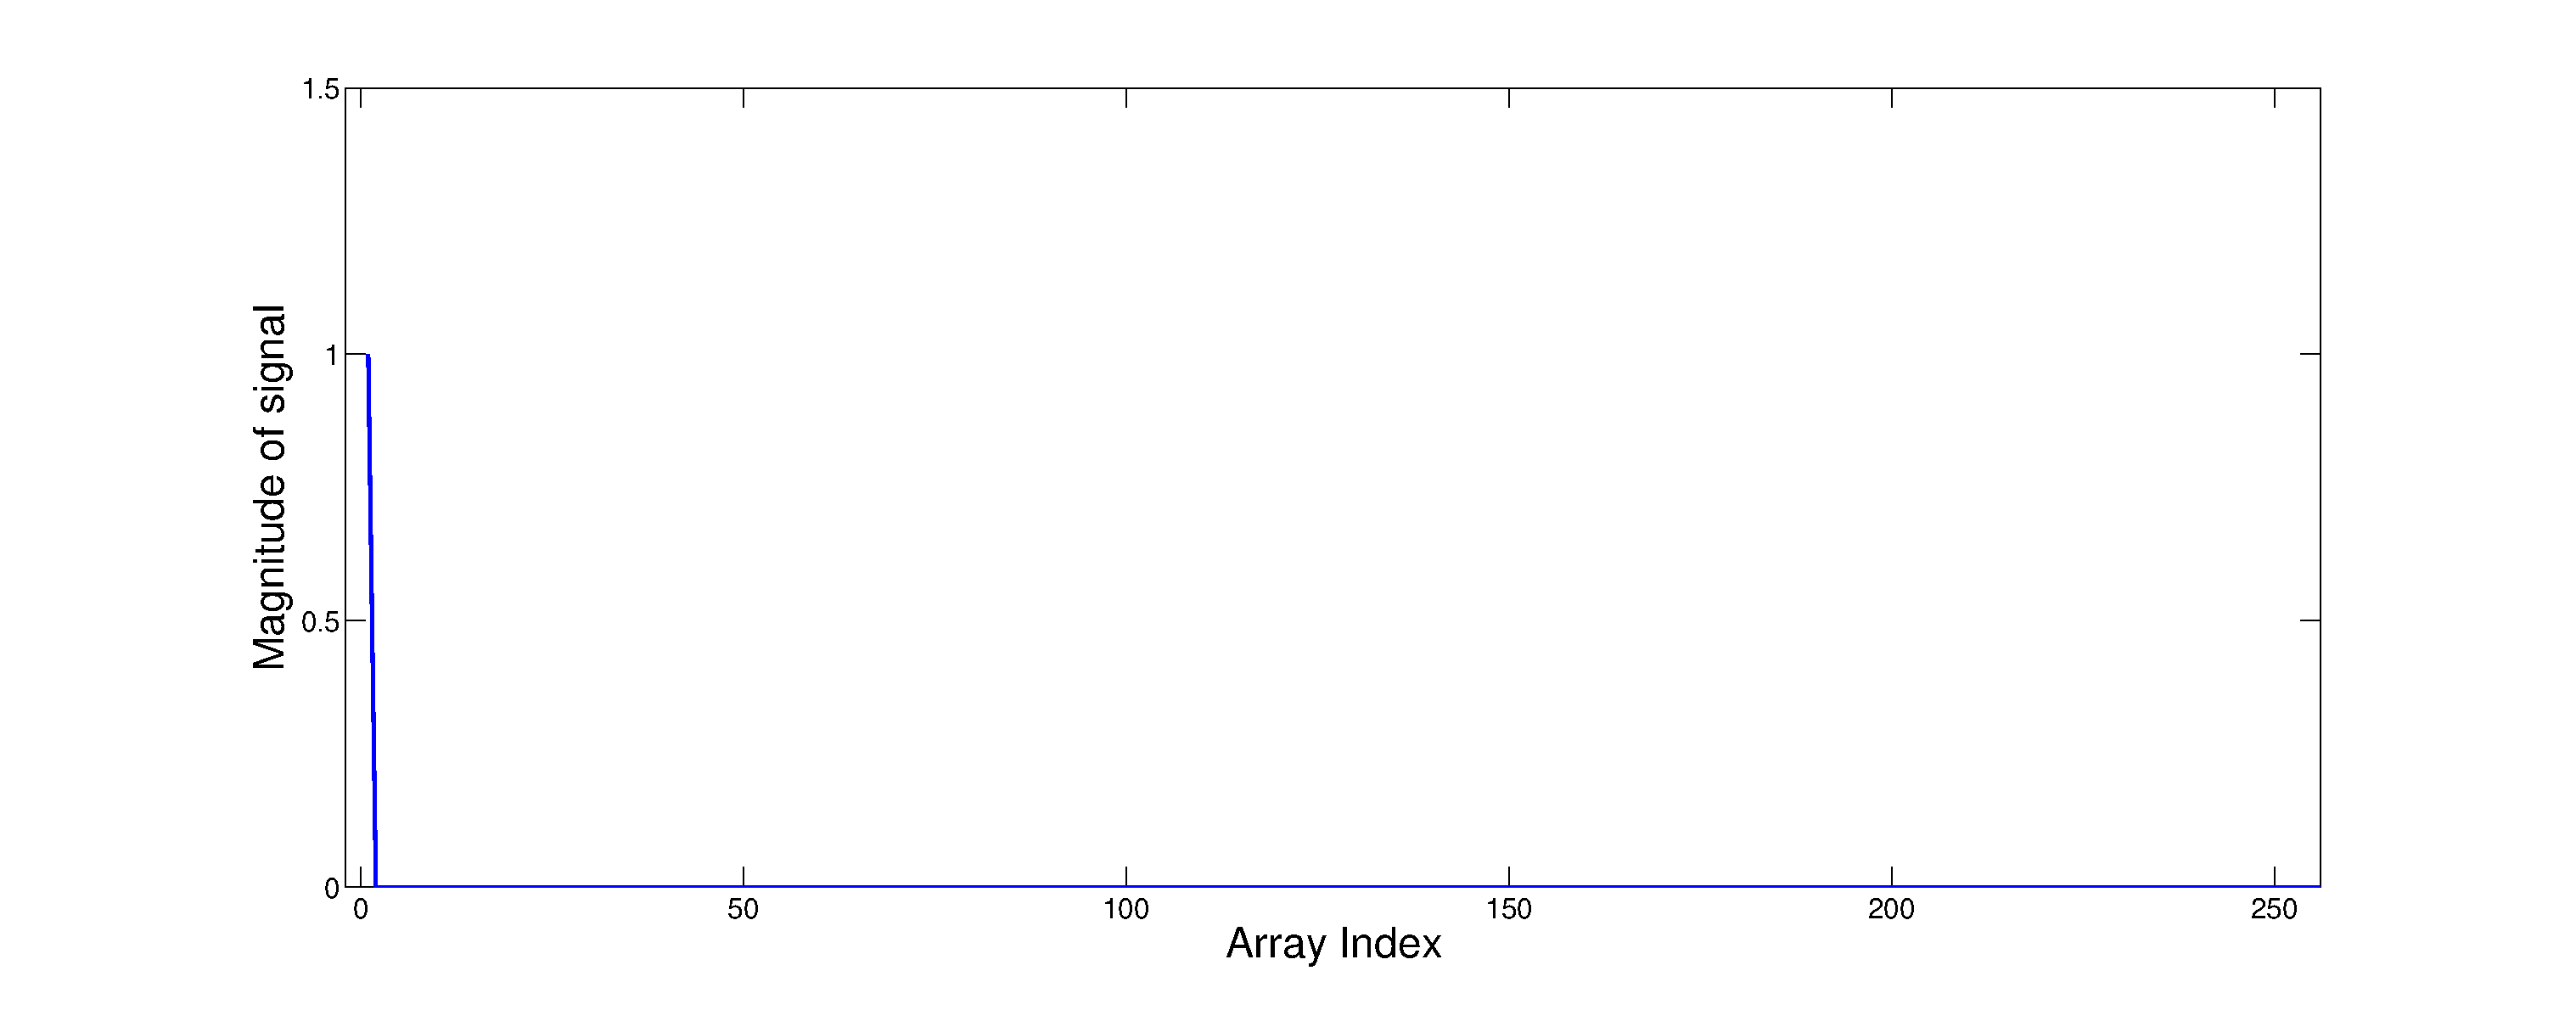
\includegraphics[width=\textwidth]{./Figures/AVR_FFT_Dirac_Input.eps}
\caption{Input Dirac Signal for AVR fast Fourier transform}
\label{fig:AVR:FFT:Dirac:Input}
\end{figure}
\begin{figure}
\subfigure[Magnitude of the Complex Output from the AVR\label{fg:Square2D:Signal}]{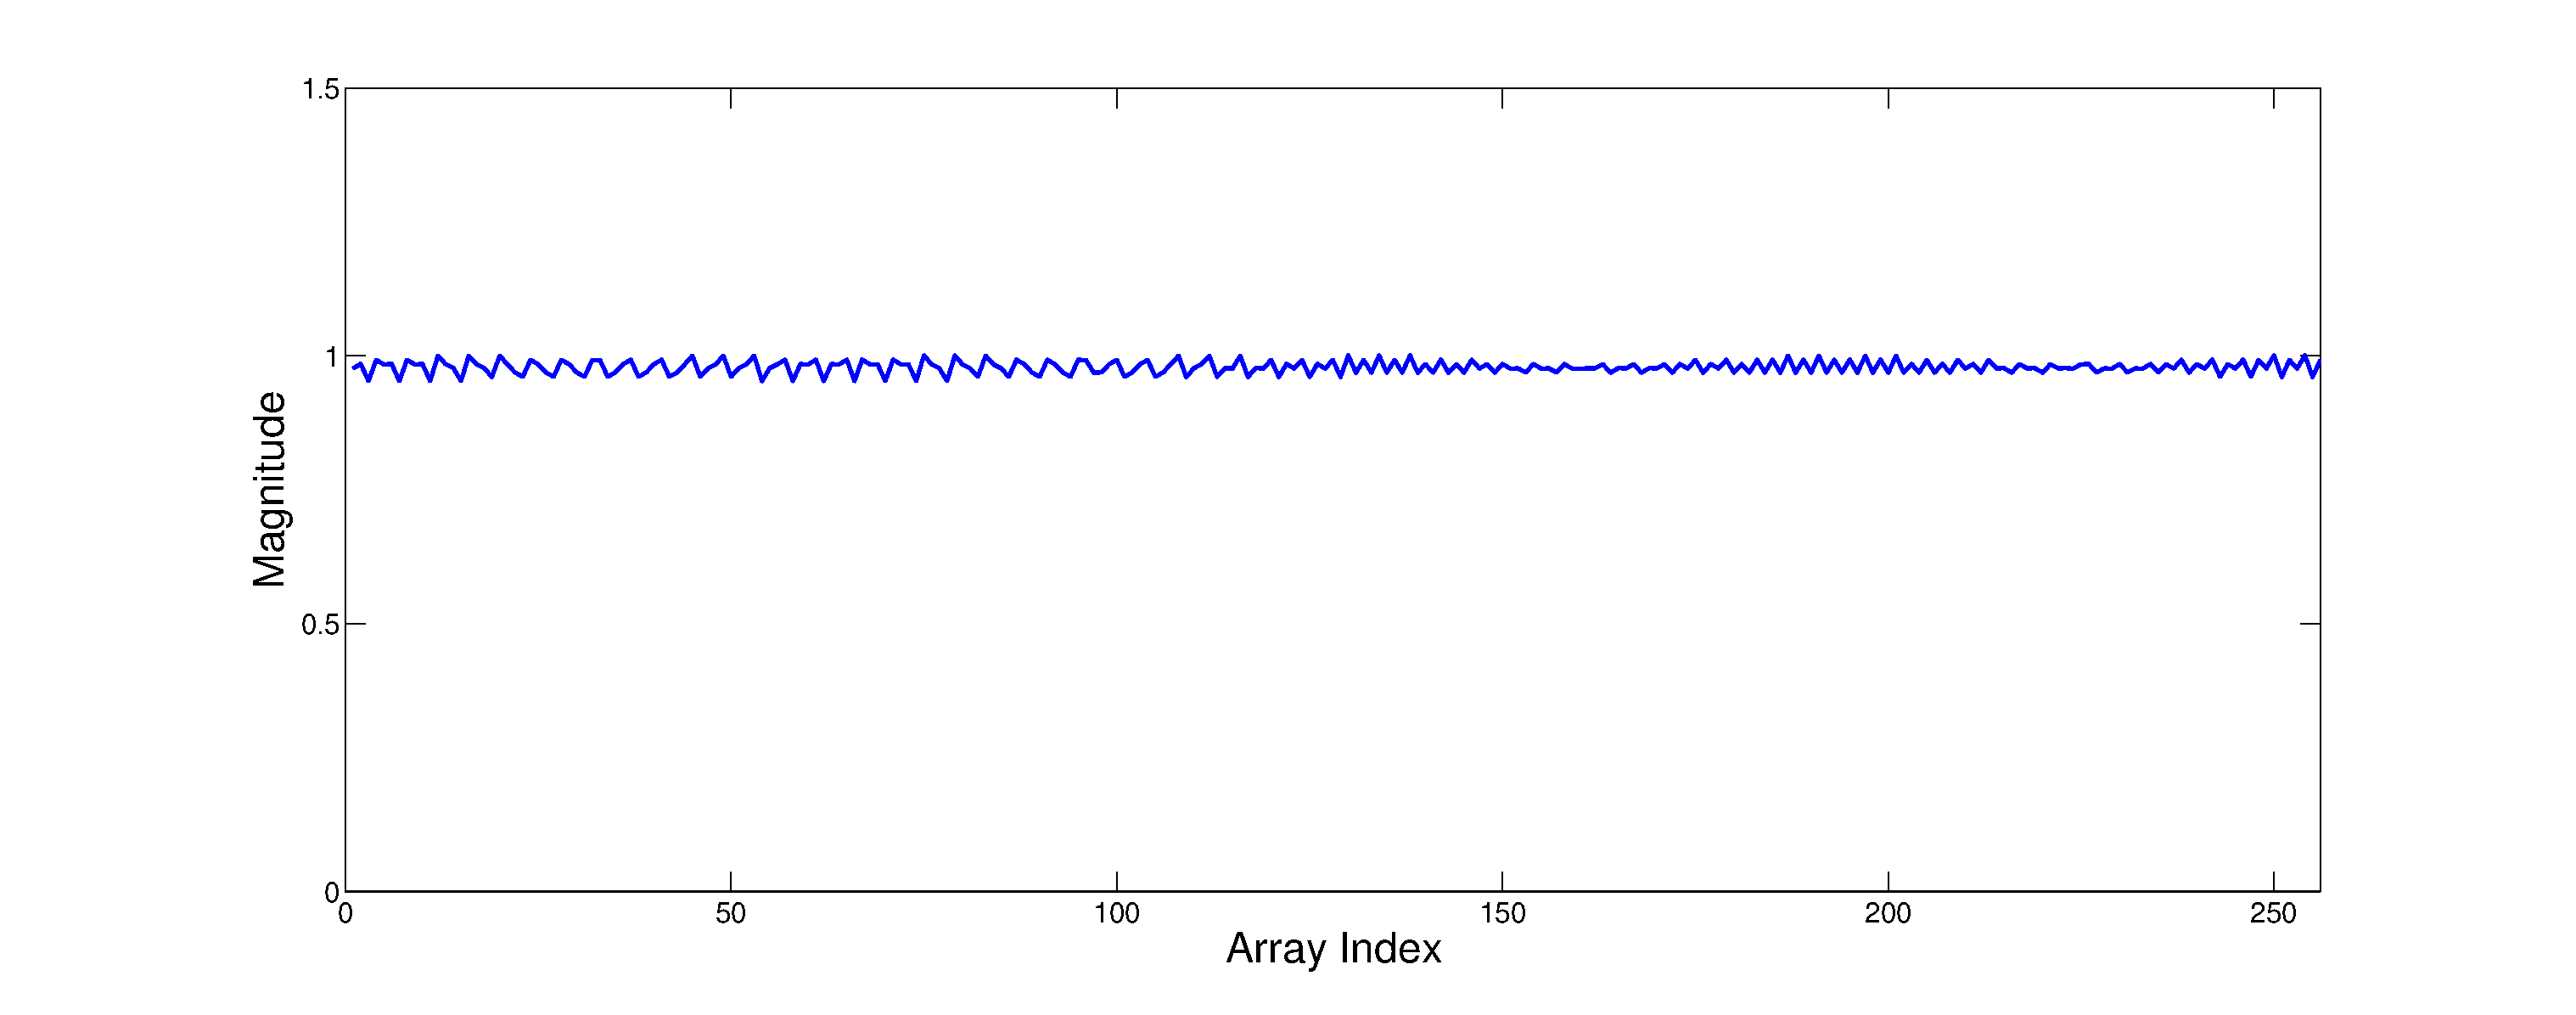
\includegraphics[width =\textwidth, keepaspectratio]{./Figures/AVR_FFT_Dirac_Complex_Mag.eps} }
\subfigure[Phase of the Complex Output from the AVR\label{fg:Square2D:Signal}]{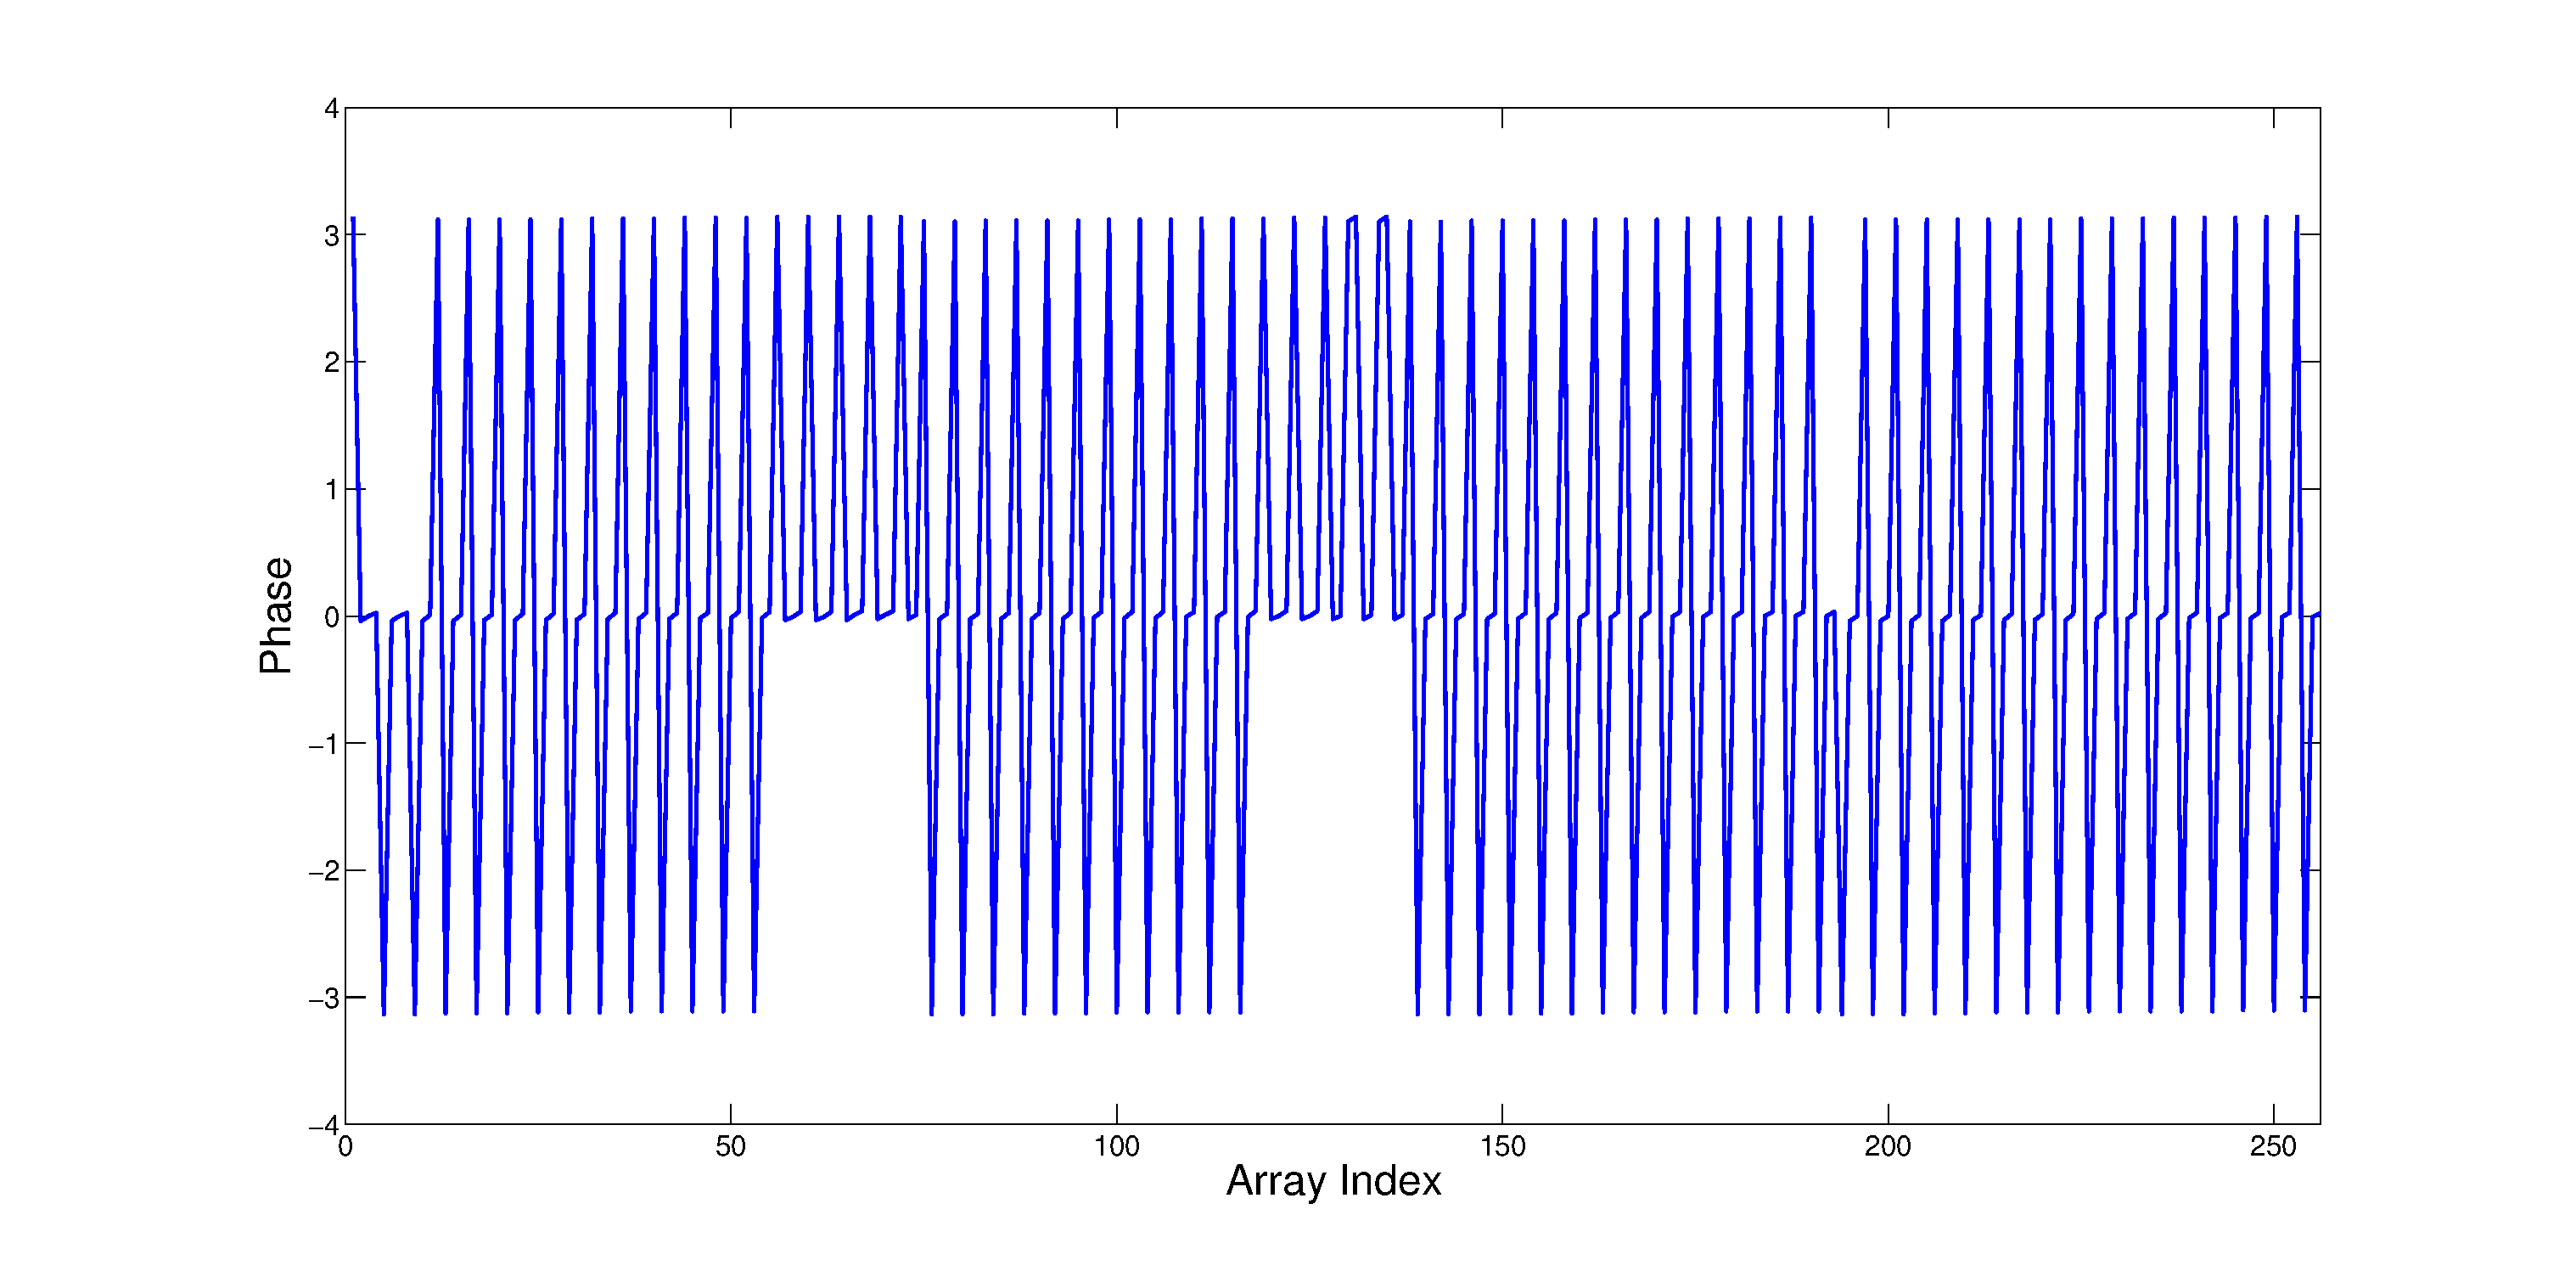
\includegraphics[width =\textwidth, keepaspectratio]{./Figures/AVR_FFT_Dirac_Complex_Phase.eps} }
\caption{Output phase and magnitude of the complex output from AVR fast Fourier transform of a Dirac function}
\label{fig:AVR:FFT:Dirac:Output}
\end{figure}

\begin{figure}
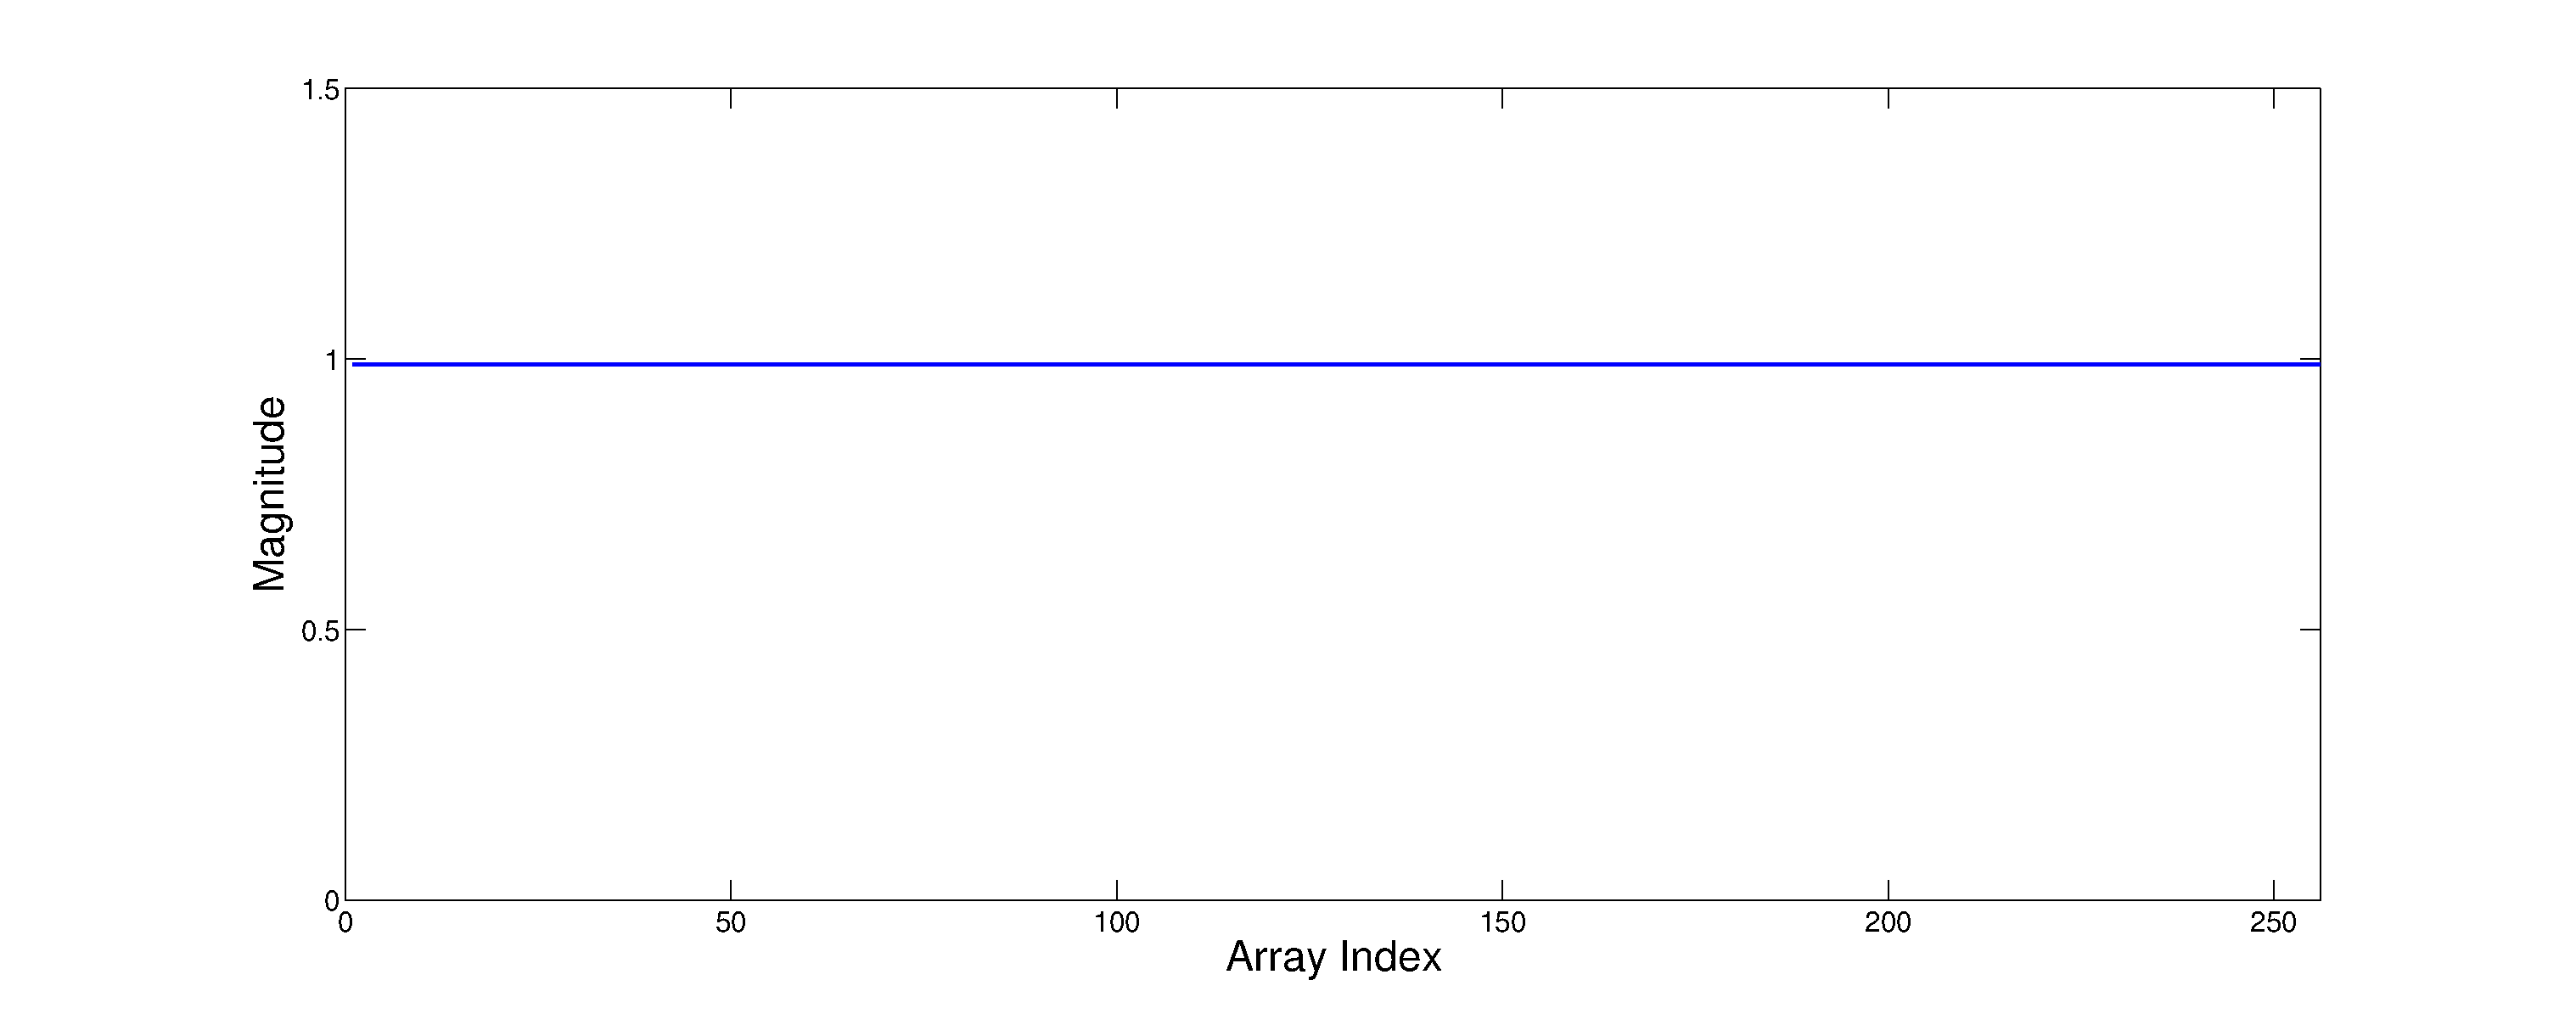
\includegraphics[width=\textwidth]{./Figures/AVR_FFT_Dirac_Mag.eps}
\caption{Magnitude calculated by the AVR of the Fourier transform of a Dirac function}
\label{fig:AVR:FFT:Dirac:Mag}
\end{figure}

\begin{figure}
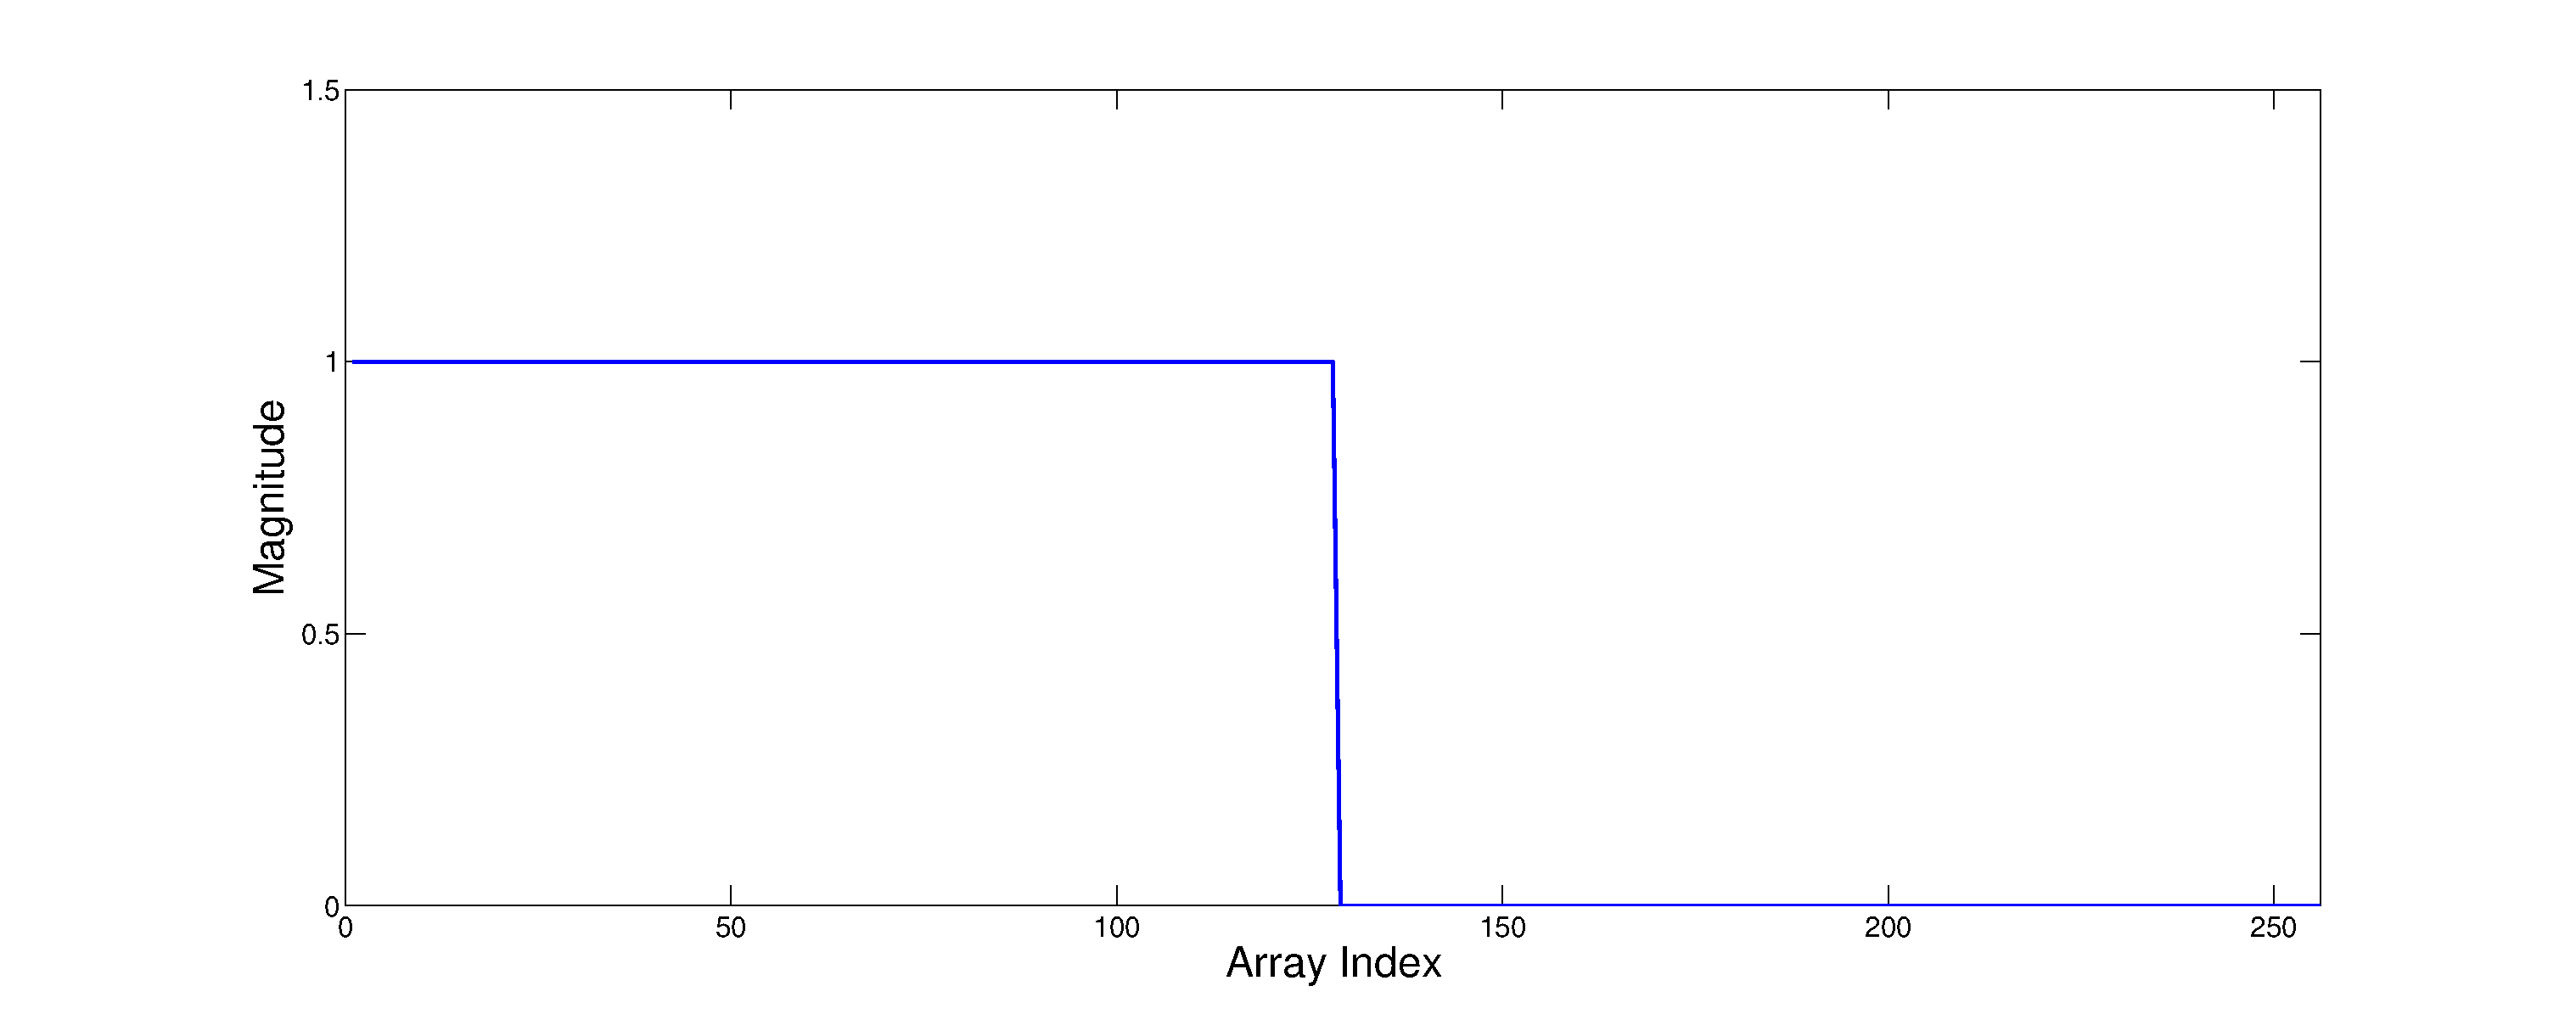
\includegraphics[width=\textwidth]{./Figures/AVR_FFT_Square_Input.eps}
\caption{Input Rectangular Pulse for AVR fast Fourier transform}
\label{fig:AVR:FFT:Square:Input}
\end{figure}
\begin{figure}
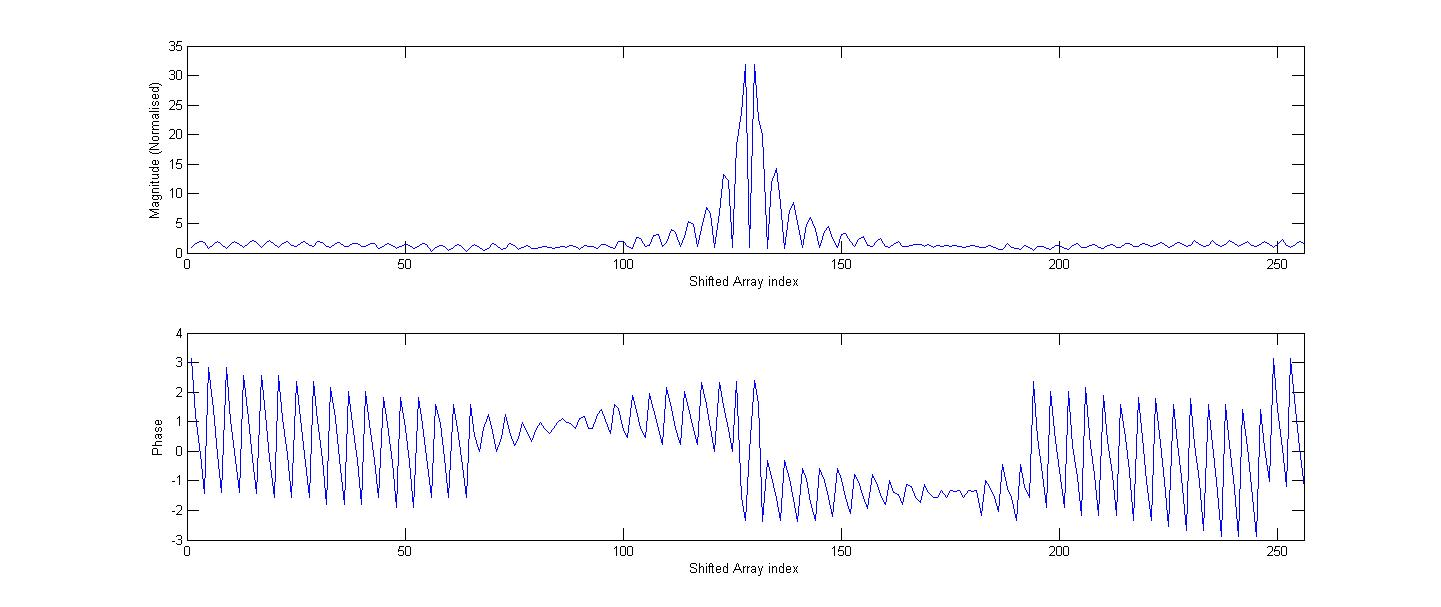
\includegraphics[width=\textwidth]{./Figures/AVR_FFT_Square_Complex_Output.jpg}
\caption{Output phase and magnitude of the complex output from AVR fast Fourier transform of a Rectangular Pulse}
\label{fig:AVR:FFT:Square:Output}
\end{figure}
\begin{figure}
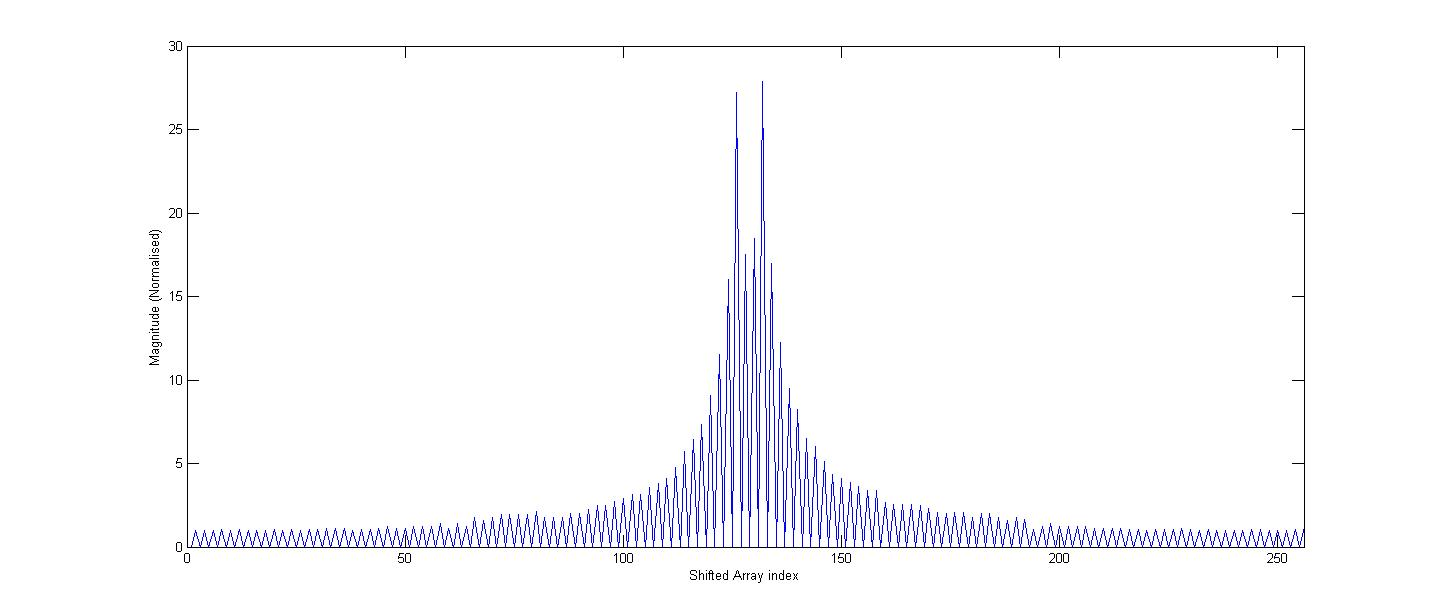
\includegraphics[width=\textwidth]{./Figures/AVR_FFT_Square_Mag.jpg}
\caption{Magnitude calculated by the AVR of the Fourier transform of a Rectangular Pulse}
\label{fig:AVR:FFT:Square:Mag}
\end{figure}

\subsubsection{2D FFT Test}

Two test signals were used to test the 2D FFT on the AVR, a Dirac signal and a square wave, seen in figures \ref{fg:Dirac2D:Signal} and \ref{fg:Square2D:Signal}. The internal method on the AVR was not able to compute the magnitude due to the method scaling all the values down causing truncation errors. The complex Fourier transform was obtained, saved to the SD card in CSV format and viewed in MATLAB. All data was normalised to omit the effects of the fixed point notation and the data shifted so that frequency 0 is in the centre. These test were done with a $64\times64$ 2D data as with a $256 \times 256$ array, the AVR runs out of internal RAM to calculate the transform. 
\inote{I would like to get this to work by the end but not vital.}

The result of the Dirac test is seen in figure \ref{fig:AVR:FFT2:Dirac}. A similar error is found in the magnitude, but the spectrum is generally flat with a small amount of ripple as seen with the 1D FFT in figure \ref{fig:AVR:FFT:Dirac:Mag}. The phase has similar issues as with the 1D FFT. However, there appears to be the correct pattern with the 2D phase, but rotated about $45^{\circ}$. This is also the case with the square wave test. The magnitude in figure \ref{fig:AVR:FFT2:Square:Mag} is very similar, with a distinct peak in the centre (frequency 0) and a sinc function extending vertically and horizontally from this. Again, however, the phase (figure \ref{fig:AVR:FFT2:Square:Phase}) seems to differ a lot from the expected result in figure \ref{fg:Square2D:Phase}. 

\subsection{Conclusion}
The transforms are calculated in real time with a 16MHz clock source. Table \ref{table:FFTSize_Time} shows the number of clock cycles taken to calculate the relevant sized transform. A $64 \times 64$ transform takes $39ms$ to compute with a 16MHz clock. This could be reduced by increasing the internal clock speed on the AVR, potentially taking it up to 33MHz and therefore halving the time to compute. A $64 \times 64$ image, however, is not practical for the application. Larger transforms can be done, but further development is required, especially to use the RAM more efficiently.%more effort needs to be taken and the external RAM could be utilised more effectively.

%\begin{table}
%\caption{Number of clock cycles taken to calculate the Transform of 64 or 256 long data set}
%\begin{tabular}{|c|c|c|c|} \cline{2-4}
%\multicolumn{2}{c|}{ } & \multicolumn{2}{|c|}{ Size of FFT } \\ \cline{2-4}
%\multicolumn{2}{c|}{ } & 64 & 256 \\ \hline
%\multirow{2}{*}{Number of Dimensions} 	&	1 	&	5019 	& 	23599		\\
%										& 	2 	& 	618168 	& 	Not Done 	\\ \hline
%\end{tabular}
%\end{table}
\begin{table}
\centering
\caption{Number of clock cycles taken to calculate the Transform of 64 or 256 long data set}
\label{table:FFTSize_Time}
\begin{tabular}{|c|c|c|c|} \cline{2-3}
\multicolumn{1}{c|}{ } & \multicolumn{2}{|c|}{ Size of FFT Data } \\ \cline{2-3}
\multicolumn{1}{c|}{ } & 64 & 256 \\ \hline
					1D 	&	5019 	& 	23599		\\ \hline
				 	2D 	& 	618168 	& 	- 	\\ \hline
\end{tabular}
\end{table}

\begin{figure}
\subfigure[A 3D Plot of the normalised magnitude of the complex data returned by the 2D fast Fourier Transform on the AVR \label{fig:AVR:FFT2:Dirac:Mag}]{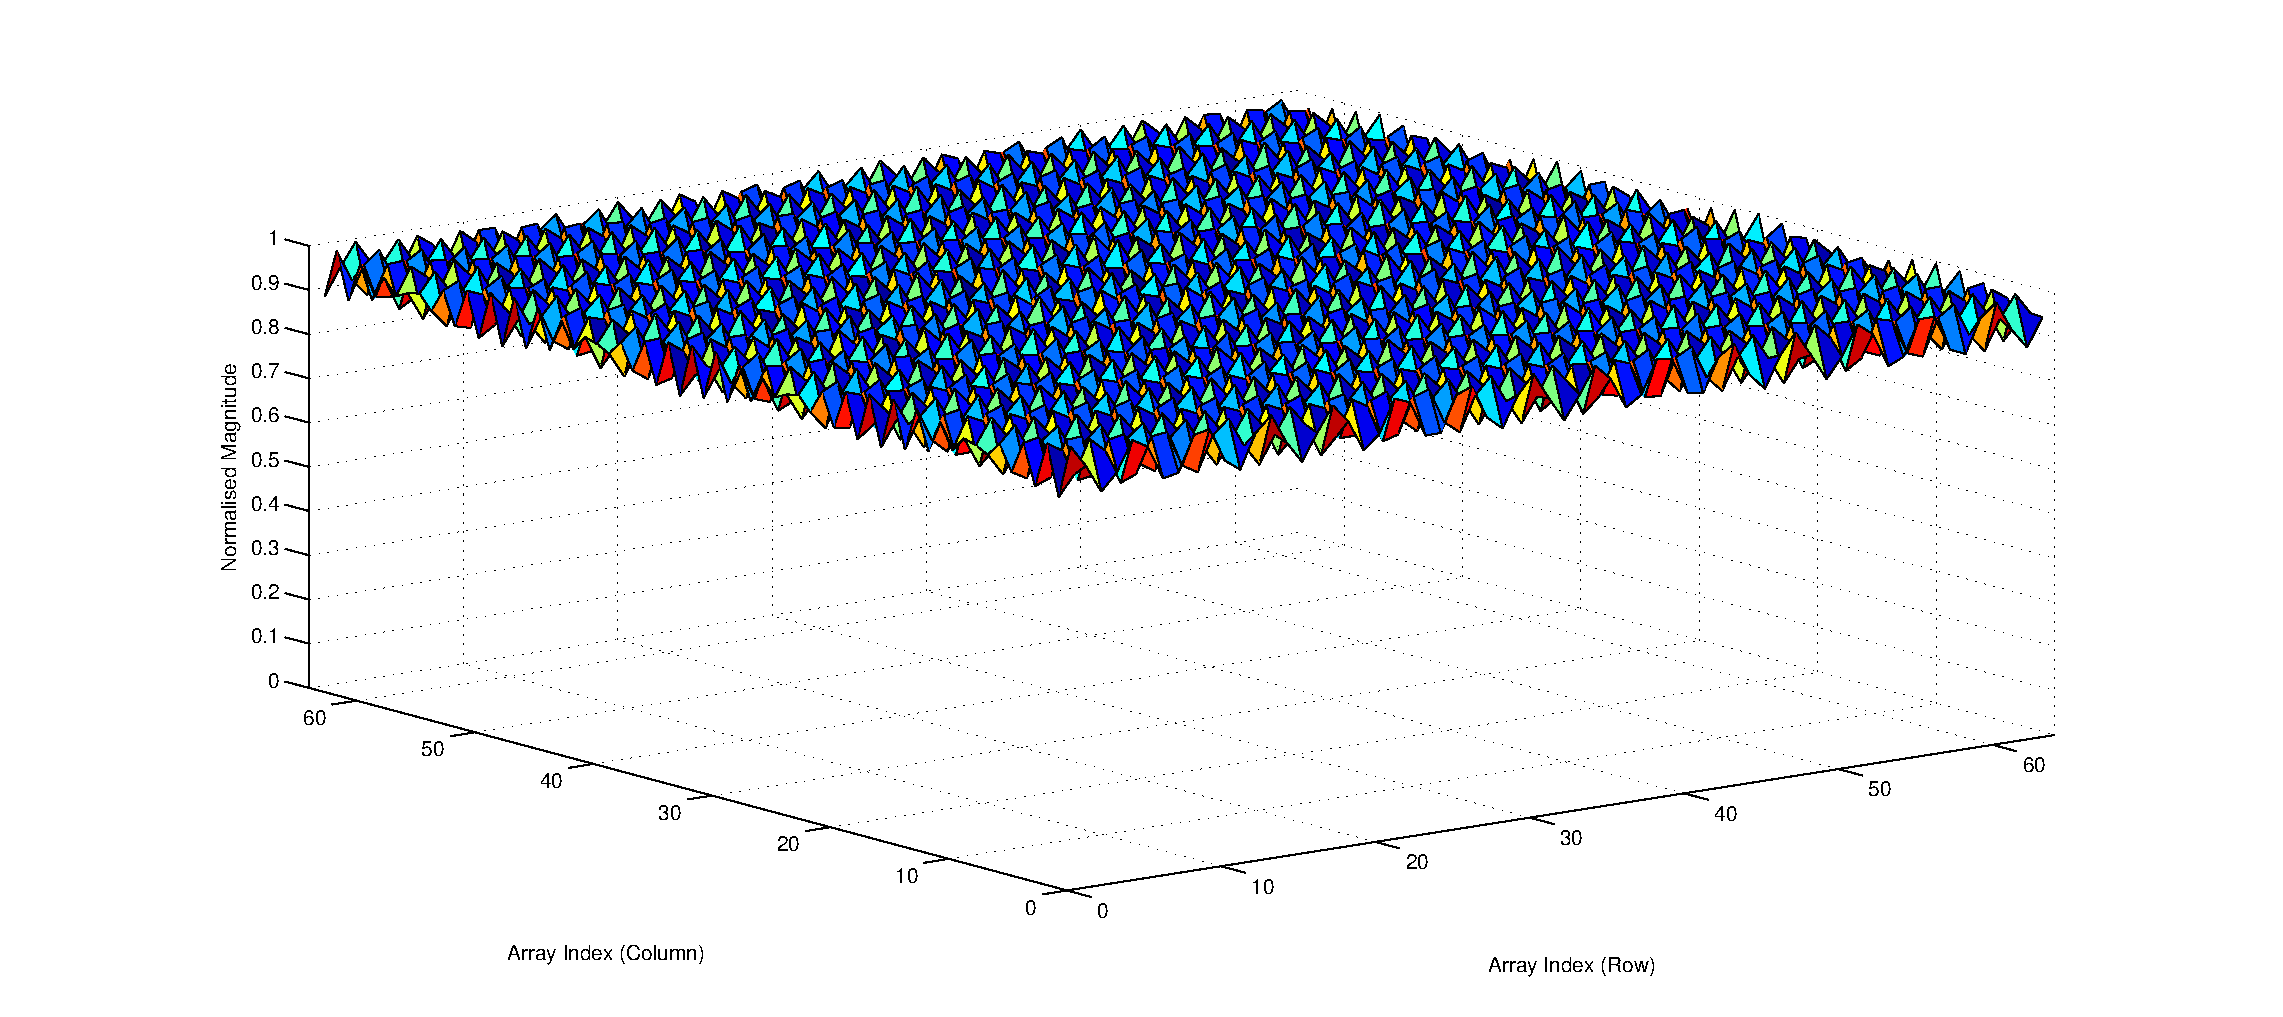
\includegraphics[width=\textwidth]{Figures/AVR_FFT2_Dirac_Mag.eps}}
\subfigure[A 3D Plot of the phase of the complex data returned by the 2D fast Fourier Transform on the AVR \label{fig:AVR:FFT2:Dirac:Phase}]{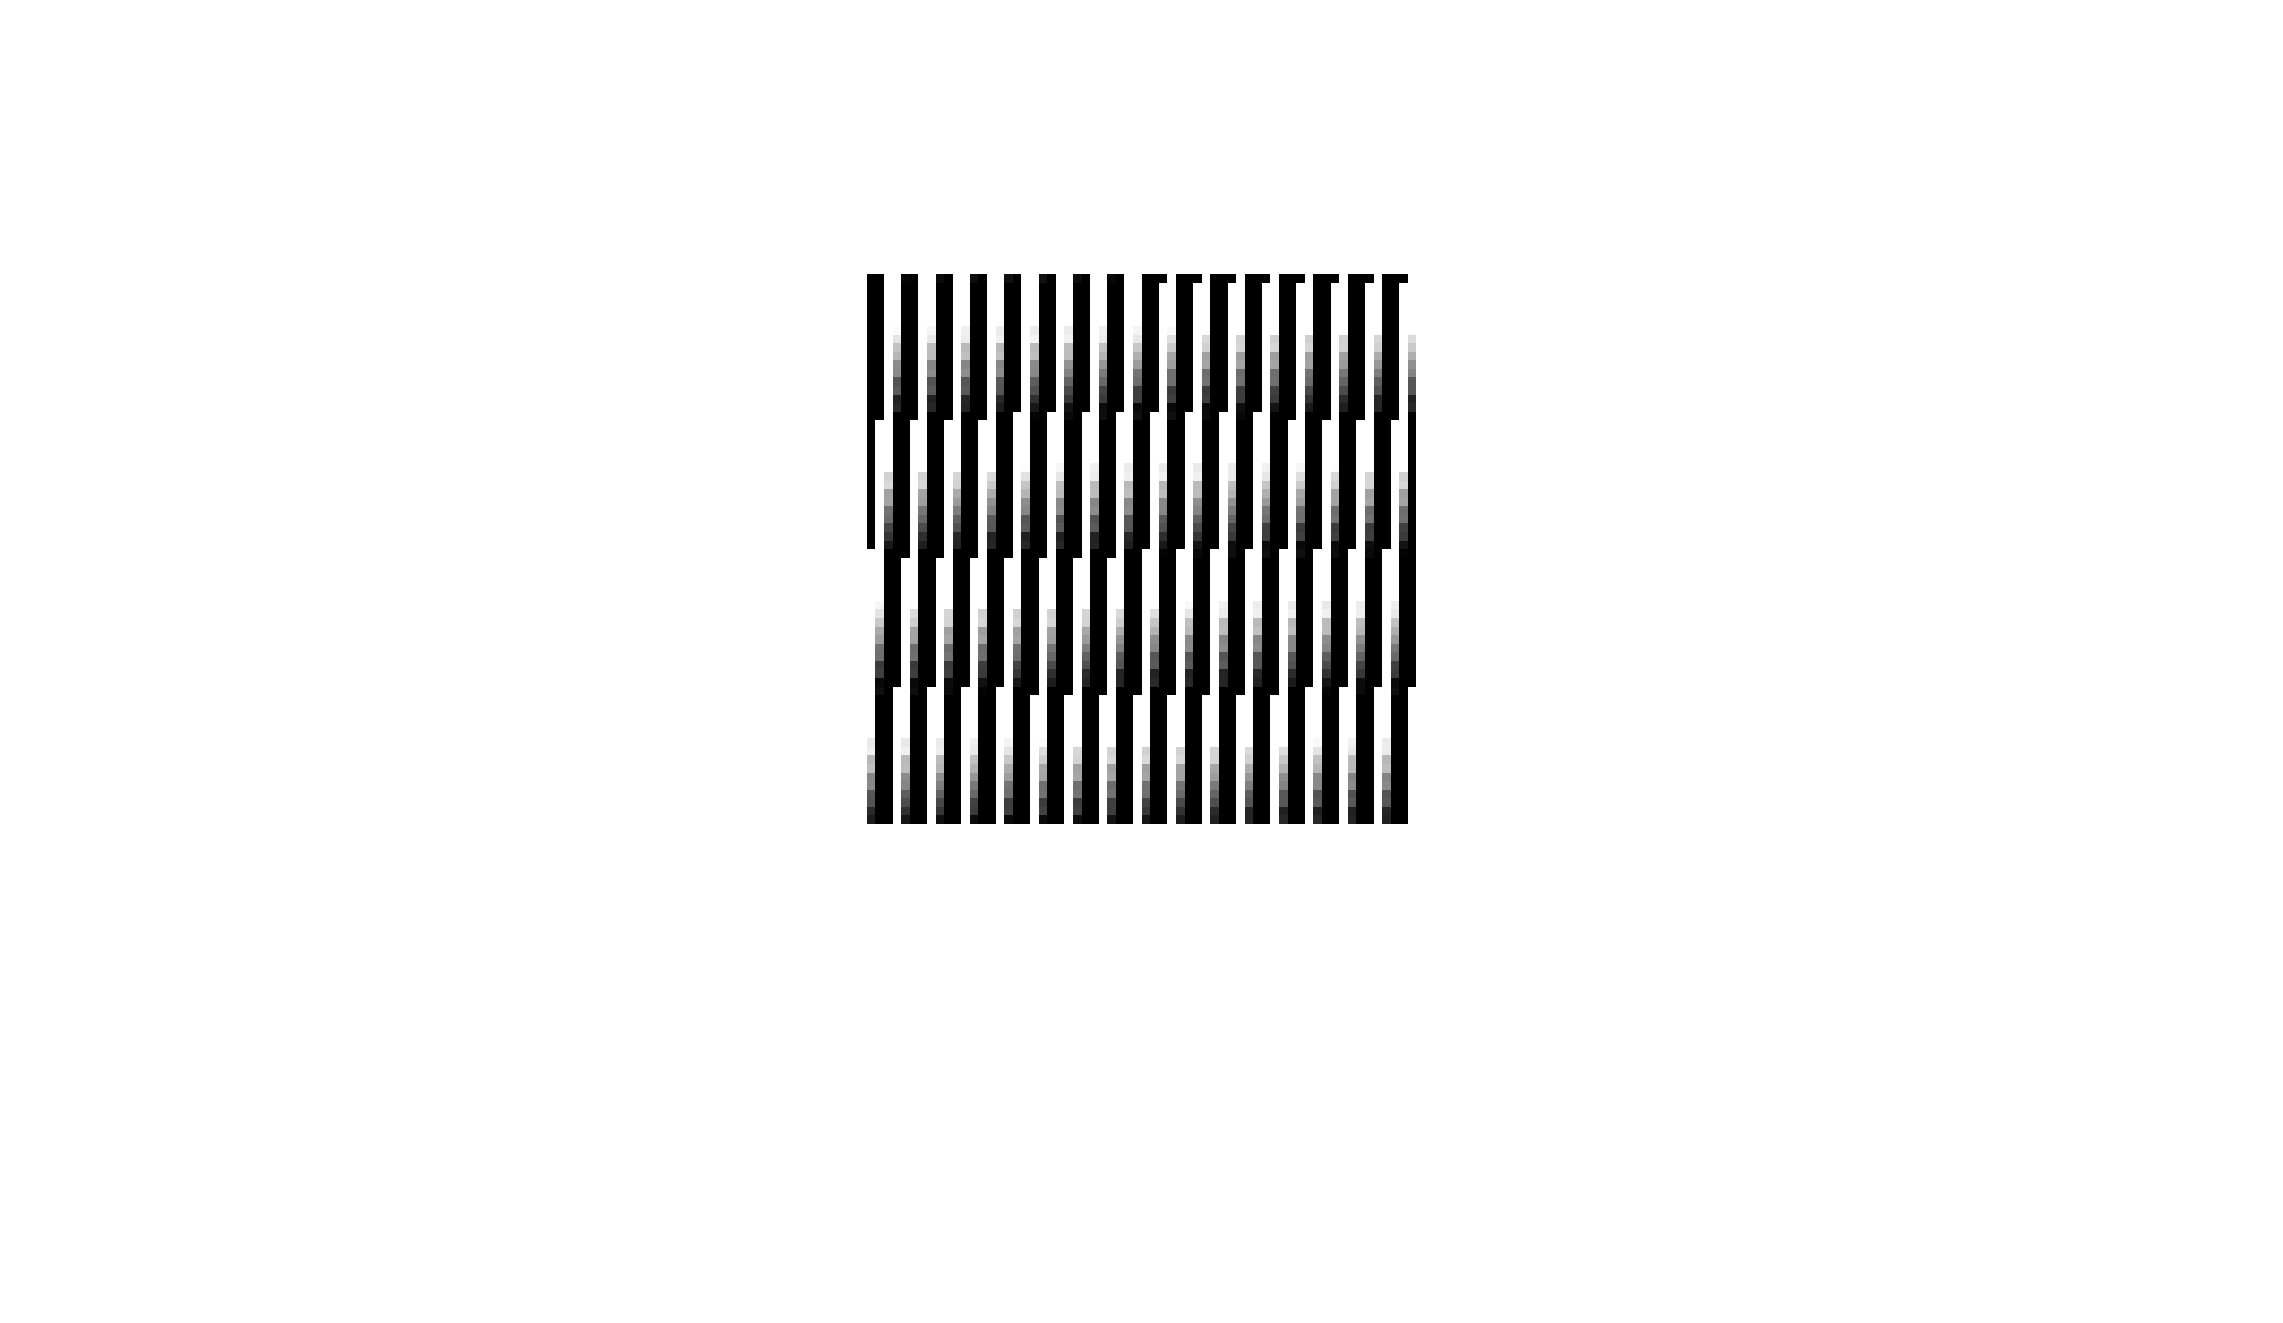
\includegraphics[width=\textwidth]{Figures/AVR_FFT2_Dirac_Phase.eps}}
\caption{3D Plots of the phase and magnitude of the Complex Data returned from the 2D FFT on the AVR of a 2D Dirac Function}
\label{fig:AVR:FFT2:Dirac}
\end{figure}

\begin{figure}
\subfigure[A 3D Plot of the normalised magnitude of the complex data returned by the 2D fast Fourier Transform on the AVR \label{fig:AVR:FFT2:Square:Mag}]{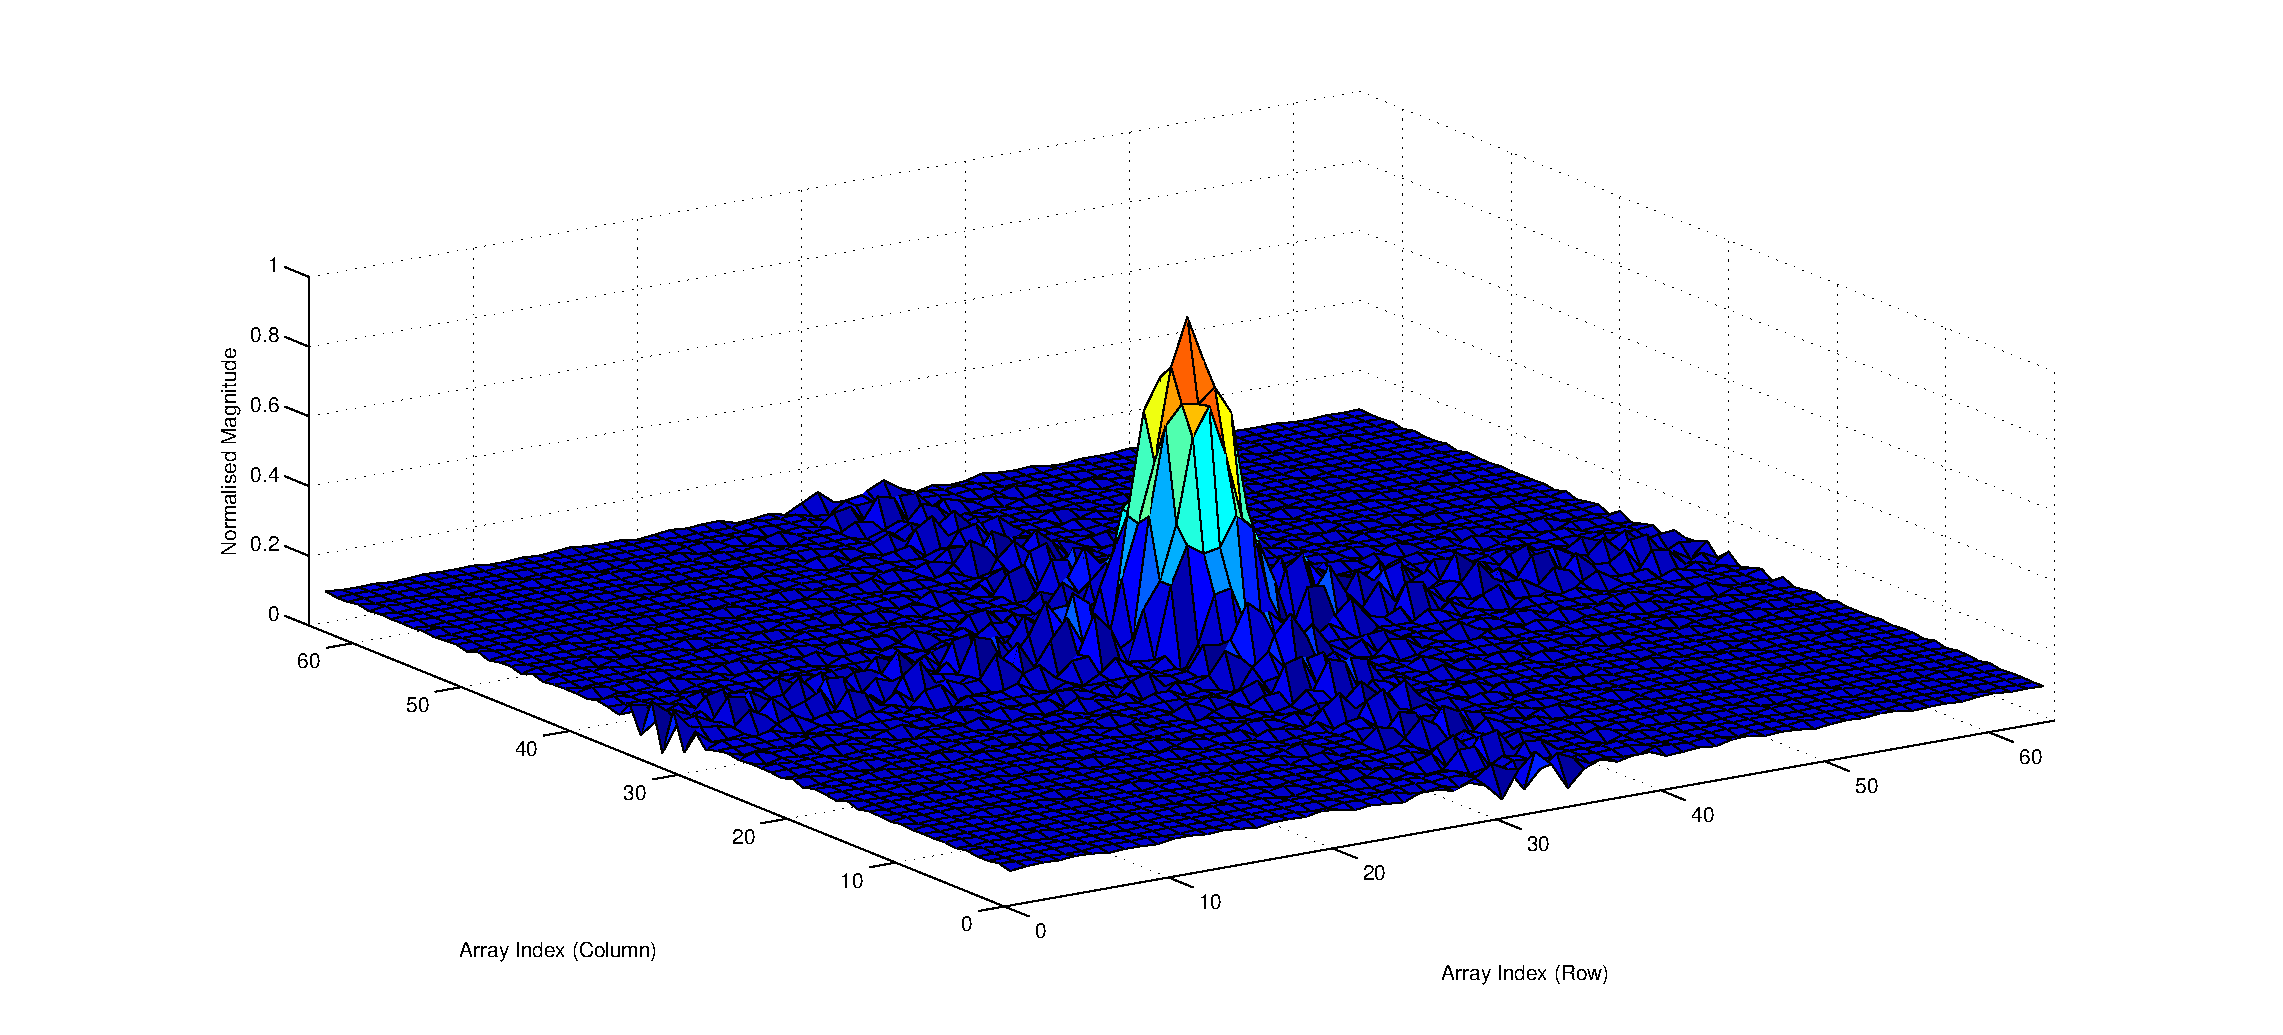
\includegraphics[width=\textwidth]{Figures/AVR_FFT2_Square_Mag.eps}}
\subfigure[A 3D Plot of the phase of the complex data returned by the 2D fast Fourier Transform on the AVR \label{fig:AVR:FFT2:Square:Phase}]{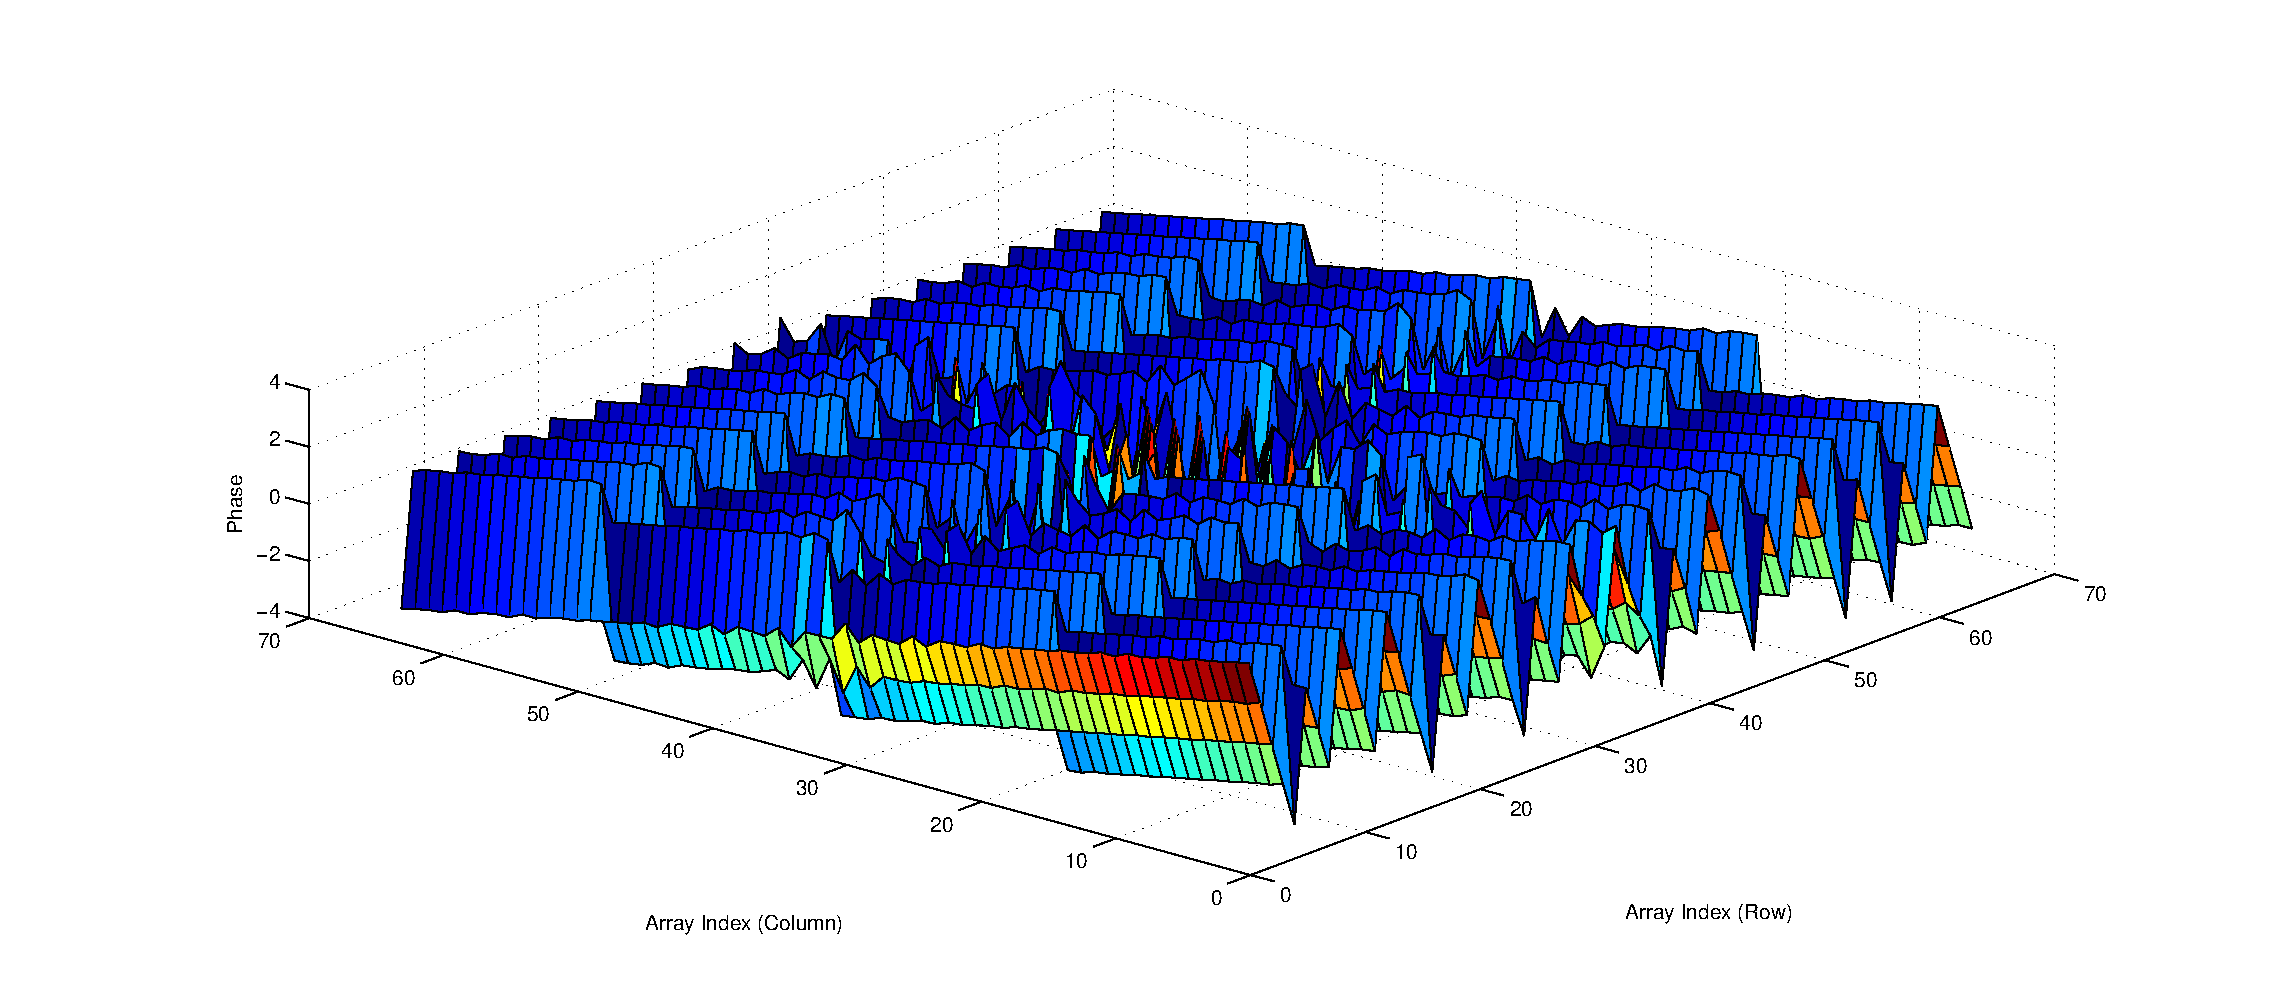
\includegraphics[width=\textwidth]{Figures/AVR_FFT2_Square_Phase.eps}}
%\subfigure[Figure \ref{fig:AVR:FFT2:Square:Mag} shown as a grey scale image\label{fig:AVR:FFT2:Square:Mag:Image}]{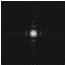
\includegraphics[width=(\textwidth / 2)]{Figures/AVR_FFT2_Square_Mag_Image.jpg}}
%\subfigure[Figure \ref{fig:AVR:FFT2:Square:Phase} shown as a grey scale image\label{fig:AVR:FFT2:Square:Phase:Image}]{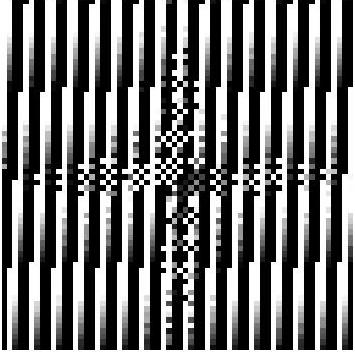
\includegraphics[width = (\textwidth / 2)]{Figures/AVR_FFT2_Square_Phase_Image.jpg}}
\caption{3D Plots of the phase and magnitude of the Complex Data returned from the 2D FFT on the AVR of a 2D Square Function}
\label{fig:AVR:FFT2:Square}
\end{figure}

\inote{Show results of actual photo being transformed, need 2D 256 FFT working before}
\inote{Maybe IFFT it too to find total errors in algorithm?}
%\section{Low Level Vision Algorithms}
%\subsection{Noise Reduction}
%\inote{Why}
%Noise exists in all signals. Two noise sources for the camera image is random noise in the sensor, and quantisation noise. It generates a compromise between noise and resolution that has to be made. Large amounts of noise reduction will blur edges and therefore reduce the quality of the image and make it harder to match. This section will investigate some noise reduction methods, and test if the application of them increases the reliability of matching using the Normalised Cross Correlation method discussed in section \ref{Section:NCC}. 
%\inote{Theory}
%\inote{Examples}
%\inote{Does it improve the reliability of matching? Vary noise amount in images? and test}
%\subsection{Edge Detection}
%\inote{Why}
%\inote{Theory}
%\inote{Examples}
%\inote{Does it improve the reliability of matching?}
